\documentclass{report}
\usepackage{hyperref}
\usepackage{amsmath}
\usepackage{amssymb}
\usepackage{amsthm}
\usepackage{listings}
\usepackage{parskip}
\usepackage{graphicx}
\usepackage{hyphenat}
\usepackage{xurl}
\usepackage[center]{caption}

\newcommand\imagewidth{\textwidth}

\newcommand\sds{\spacefactor\sfcode`.\ \space}

\hyphenation{I-THINK-WERE-GO-ING-CRA-ZY}
\hyphenation{DAN-CING-ON-THE-ROOF-SHOOT-ING-HOLES-IN-THE-MOON}
\hyphenation{BROKE-DOWN-OUT-IN-A-DITCH-OF-OLD-RUB-BISH}
\hyphenation{THROW-THOSE-PIC-TURES-DOWN-THE-LANE}
\hyphenation{JU-DAS-TRAIN-WRECK}
\hyphenation{JU-DAS-TRAIN-WRECK-NO-HAN-DLE-BARS}

\newtheorem{thm}{se lojysra}
\renewcommand*{\proofname}{lojysra}
\title{+/ Drawings}
\author{la .varik.\ .VALefor.}
\begin{document}
\maketitle{}
\tableofcontents{}
\chapter{le terfi'i}
ni'o la'o gy.\ +/ Drawings .gy.\  cu vasru ko'a goi le su'o lampru pixra be fi la .varik.\ .VALefor.\ ge'u je le datni be ko'a

.i pilno zo su'o ki'u le nu su'o da poi ke'a pixra fi la .varik.\ .VALefor.\ zo'u selcaugau da la'o gy.\ +/ Drawings .gy.\sds  .i mupli fa le nu selcaugau lo glefi'a be fi la .varik.\ la'o gy.\ +/ Drawings .gy.

\chapter{le plijaspu}
ni'o so'i da poi ke'a pixra je cu se zbasu la .varik.\ je cu selvau ko'a goi la'o gy.\ +/ Drawings .gy.\ zo'u le velski be da cu xusra le du'u la'o gy.\ CC BY-NC 4.0 .gy.\ cu plijaspu da\sds  .i ku'i ro da poi ke'a pixra je cu se zbasu la .varik.\ je cu selvau ko'a zo'u la .varik.\ pu gasnu le nu la'oi .Unlicense.\ cu plijaspu da\sds  .ija'e ro da poi ke'a pixra je zu se zbasu la .varik.\ je cu selvau ko'a zo'u la'oi .Unlicense.\ cu plijaspu da

\chapter{la'o gy.\ 20200414042645-03 .gy.}
\begin{figure}[ht]
	\centering
	
\includegraphics[keepaspectratio, width=\textwidth, height=0.75\textheight]{20200414042645-03/20200414042645-03.jpg}
	\caption[center]{le ciplanli pixra noi ke'a claxu lo xamgu je cmene}
\end{figure}
\section{le pamoi ve skicu be le pixra}
ni'o pu zbasu le pixra ki'u le nu djica lo nu facki lo jei me'oi .viable.\ fa lo nu pilno lo sma'aci lo nu pixra kei kei je lo jei la'oi .GIMP.\ xlali samru'e\sds  .i la .varik.\ cu terxra ca le nu le mutce be le ka ce'u filselga'e cu selbi'o le su'u la'oi .GIMP.\ cu mutce le ka ce'u xlali kei kei je le jei me'oi .viable.\ fa lo nu pilno lo sma'aci lo nu pixra

ni'o nelci lo diksiseli

\section{le me'oi .watermark.}
ni'o la .varik.\ cu jinvi le du'u le me'oi .watermark.\ po le pixra cu dukse\ldots\sds  .i di'u mutce le ka ce'u jetnu kei ca le nu la .varik.\ cu pensi le du'u la .varik.\ cu pu fairgau lo favytcinymupli be fi le pixra poi claxu le me'oi .watermark.

\begin{figure}[ht]
	\centering
	
\includegraphics[width=10cm]{20200414042645-03/20200414042645-03-uw.png}
	\caption[center]{ni'o gubyternoi lo favytcinymupli be le pixra\ldots be'o poi ke'a claxu lei kerfa tengu\sds  .i rigni}
\end{figure}

\section{le cfila be la'o gy.\ 20200414042645-03 .gy.}
ni'o cfila ko'a goi la'o gy.\ 20200414042645-03 .gy.\ fa\ldots
\begin{itemize}
	\item le su'u pixra le nu le cnebo be la'oi .\ VUNC.\ cu claxu\ldots
	\begin{itemize}
		\item lo su'o ctino be le stedu be la'oi .VUNC.\ ku ku je
		\item lo su'o sirsunla tengu kei kei je
	\end{itemize}
	\item le su'u lo ctino cu se claxu le se pixra be ko'a be'o poi galraipau le se viska pagbu be le zunle kanla be la'oi .VUNC.\ kei
\end{itemize}
vu'o po'o nai

\chapter{la'o gy.\ Proactive Security .gy.}
\begin{figure}[ht]
	\centering
	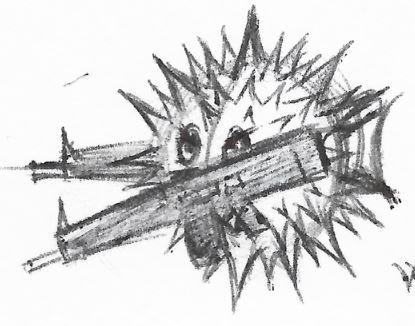
\includegraphics[width=10cm]{proactivesecurity/proactivesecurity.png}
	\caption[center]{ni'o zva'ati fa le nu mi'a pilno la'oi .OpenBSD.\sds  .i doi fazgau do'u ko na troci}
\end{figure}
\section{le pamoi velski be le pixra}
ni'o kibdu'a la'o gy.\ Proactive Security .gy.\ ki'u le nu filselga'e fa le nu claxu lo pixra be la .pyfis.

ni'o la .pyfis.\ cu claxu lo kalmebykre ki'u le nu la .su'oda.\ cu mo'ifli lo nu pixra lo kalmebykre

ni'o la'o gy.\ AA-12 .gy.\ .u'enderfu xacyce'a

\chapter{la'oi .WESTERNUNIONSOFTHECOUNTRYWESTERNS.}
\begin{figure}[ht]
	\centering
	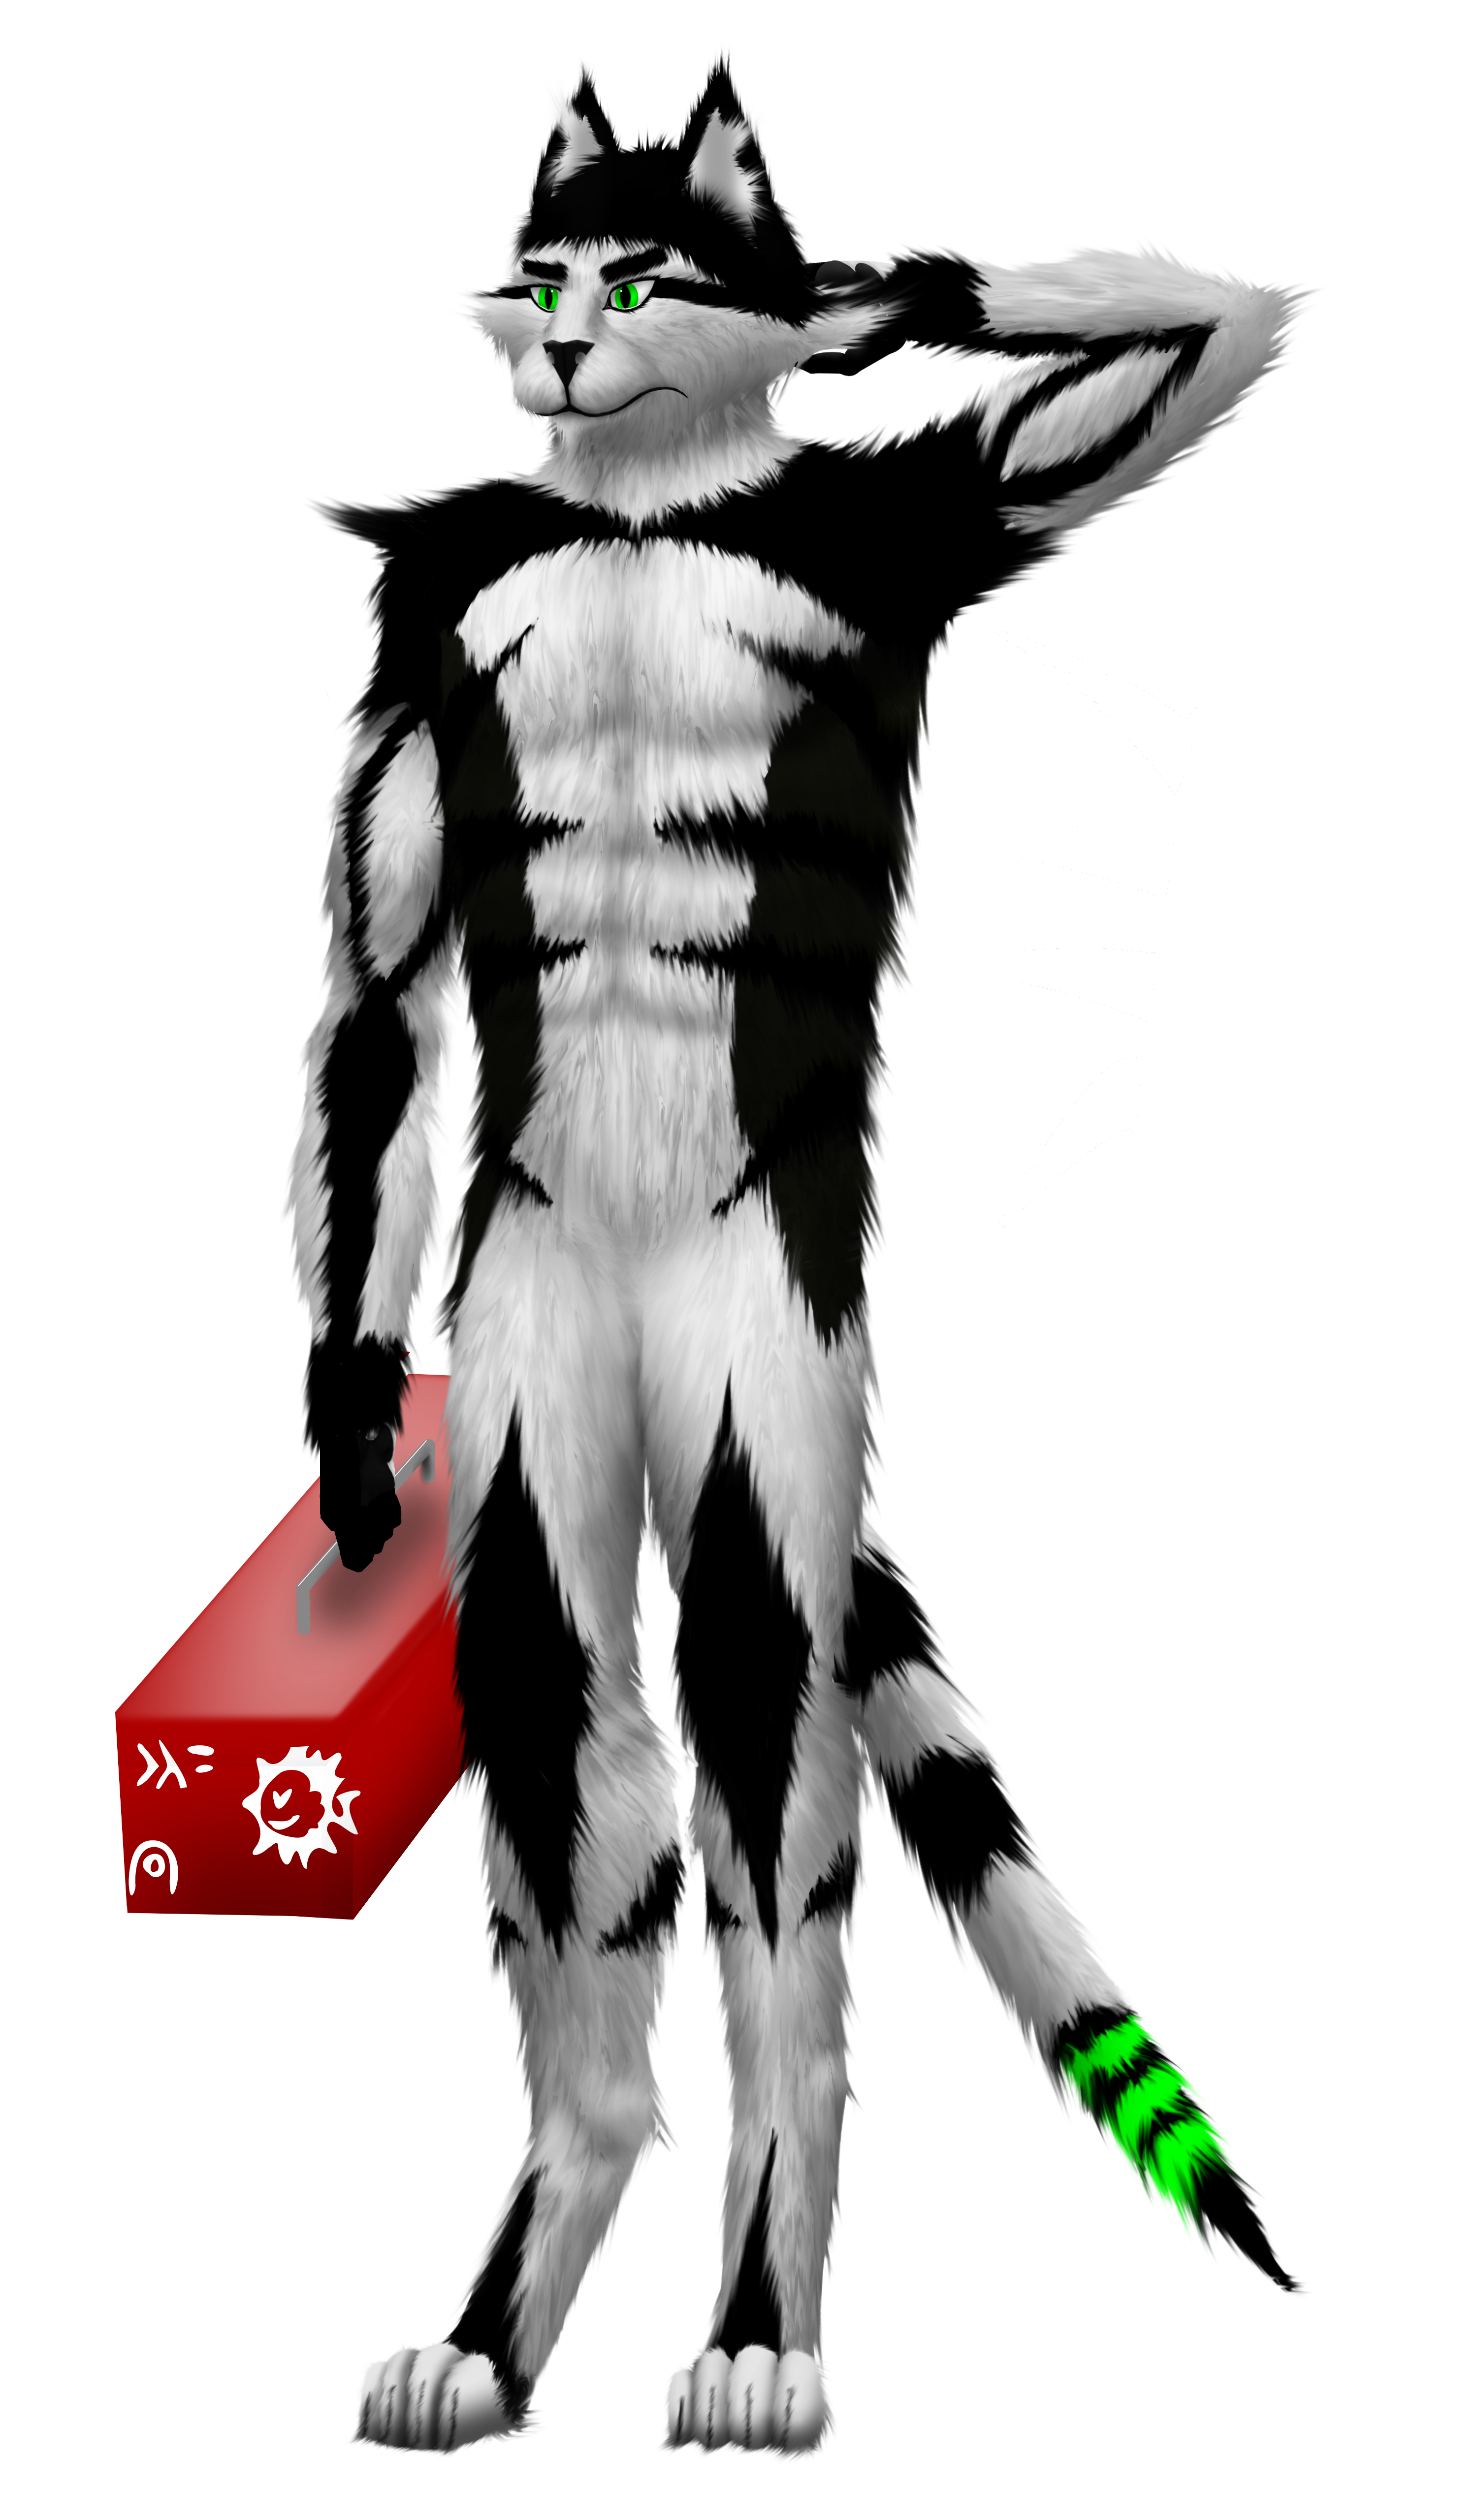
\includegraphics[keepaspectratio, width=\textwidth, height=0.75\textheight]{50x/toolbox/westernunionsofthecountrywesterns.png}
	\caption[center]{le pixra je nai lo se tcidu}
\end{figure}
\section{le pamoi velski be le pixra}
\subsection{le snada pe li ci fi'u vo}
ni'o la .varik.\ cu troci lo nu pixra lo pixra be le xarpre be la .varik.\ be'o be'o pe li ci fi'u vo kei je cu denpa fo le nu terxra kei pu le nu la .varik.\ cu pixra lo pixra be le xarpre be la .varik.\ be'o be'o pe li ci fi'u vo
\subsection{le me'oi .watermark.\ je le plijaspu}
ni'o ji'a le pixra cu na vasru lo me'oi .watermark.\ poi mutce le ka tu'a ce'u\sds  .i ku'i le pixra cu na se vasru la'o gy.\ public domain .gy.\sds  .i la .varik.\ cu ralte le krali po le pixra\sds  .i ku'i cumki fa le nu le ni di'u jetnu cu selbi'o\sds  .i le temci cu flecu pe'a ca le nu la .varik.\ cu zenba le ka ce'u djica lo nu le mu'oi gy.\ public domain .gy.\ cu vasru lo pixra be fi la .varik.

\subsection{le pilno}
ni'o pilno la'oi .Krita.\ noi mutce le ka se tolnei la .varik.

ni'o zbasu le pixra ca le nu la'oi .Krita.\ goi ko'a ge'u naru'e narpli masno\sds  .i mupli fa le du'u le nu ko'a gasnu le nu lo senta pe'a cu selvisnalka'e cu snidu li ji'i cino\sds  .i le nu masno cu pagbu rinka le nu la .varik.\ cu pilno la'oi .GIMP.\ le nu zbasu lo balvi pixra\sds  .i la .varik.\ cu ponse lo plijaspu be la'o gy.\ CLIP STUDIO PAINT EX .gy.\ je cu zmanei la'o gy.\ CLIP STUDIO PAINT EX .gy.\ la'oi .Krita.\ lo so'i krinu\sds  .i ranji zenba fa li ni'e ni la .varik.\ cu nelci la'oi .WINE.\ po la'oi .FreeBSD.

ni'o ze'i pilno la'oi .GIMP.\ pu le nu la .varik.\ cu facki le du'u la'oi .GIMP.\ claxu lo su'o jicmu poi se pilno la .varik.\sds  .i le zmiku klina senta tadji cu mupli le ka se claxu la'oi .GIMP.\sds  .i mukti le nu la .varik.\ cu pilno la'oi .Krita.\ le nu mulgau le pixra

\subsubsection{lo mu'oi zoi gy.\ open-source .gy.\ sampla cu cumki xamgu}
ni'o le mu'oi zoi gy.\ open-source .gy.\ sidbo cu se nelci la .varik\ldots je cu cumki friti lo jetnu kalci pe'a\sds  .i lu lo prenu poi to'e nelci ku'o cumki cikre lo samru'e li'u xlali krinu ki'u le nu su'o da poi pilno lo samru'e zo'u da na samru'e ciska\sds  .i ji'a lo xlali sa'u samselpla cu zasti\sds  .ije la .varik.\ cu na jinvi le du'u le samselpla po fi la'oi .Krita.\ cu cizra xamgu

ni'o le nabmi cu se mlauca ki'u le nu la .varik.\ cu djica le nu la .varik.\ cu nelci la'oi .Krita.\ je la'oi .GIMP.\sds  .i ku'i la .varik.\ cu nelci la'oi .Krita.\ je la'oi .GIMP.\  .inaja la'oi .Krita.\ je la'oi .GIMP.\ sisti le nu kalci pe'a

\subsection{le sinxa}
ni'o lo nu sispe'i le se sinxa be le sinxa cu frili lo tcidu

\subsection{le nu pilno le versiio jitro}
ni'o cumki fa le nu kibdu'a le citri be le pixra be'o la'oi .GitHub.\sds  .i la .git.\ cu jitro le pixra je cu zbasu le mlitce barda citri bo datnyveiste ki'u le nu la .varik.\ cu djica le nu la .varik.\ cu frili cple'ijdu le  .indika be le du'u la .varik.\ cu pu zbasu le pixra

\subsection{lo nu nitpiki}
ni'o mutce le ka nelci lo nu xamgu nitpiki\sds  .i ku'i la .varik.\ cu djica lo nu lo nu nitpiki cu tilcfu ki'u le nu la .varik.\ cu jinvi le du'u tu'a lu le caltai be le birka cu na mapti le ctino be le birka li'u cu zmadu tu'a lu le birka cu xlali li'u le ka filri'a lo nu xagzengau

\subsection{le selpli}
ni'o pilno la'o gy.\ ed(1) .gy.\ le nu ciska le velski poi vasru dei

\section{le cfila be le pixra}
ni'o la .varik.\ cu facki le du'u la'oi .WESTERNUNIONSOFTHECOUNTRYWESTERNS.\ goi ko'a cu xlali pixra le betfu sluji be la'oi .VUNC.\ kei je le du'u ko'a claxu le cmalu sirsunla bo tcila

\subsection{le xlali betfu bo sluji}
ni'o xlali fa le caltai be le betfu sluji be fi la'oi .VUNC.\ ku poi se pixra la'oi .WESTERNUNIONSOFTHECOUNTRYWESTERNS.

.i le nabmi cu se rinka le tadji be le nu la .varik.\ cu pixra lo betfu sluji kei ku ku goi ko'a\sds  .i ko'a pruce fo le nu pixra lo nonkansa pe'a sluji

\section{le ka ce'u claxu le tcila be lei sirsunla}
ni'o lei sirsunla po la'oi .VUNC.\ ge'u po le pixra cu nacmatilcfu

ni'o zbasu la'oi .WESTERNUNIONSOFTHECOUNTRYWESTERNS.\ ca le nu la .varik.\ cu fliba le nu jmina lo cmalu sirsunla bo tcila\sds  .i le fliba cu rinka le nu le pixra cu se vasru le barda sirsunla tcila ku po'o

\section{le sutra pirlarfi'i}
ni'o le lisri skina poi skicu le nu zbasu la'oi .WESTERNUNIONSOFTHECOUNTRYWESTERNS.\ cu kibzva la'o gy.\ \url{https://diode.zone/w/vR9yipHTfuaH3SKPiEXFLm} .gy.\ je la'o gy.\ \url{https://vimeo.com/635651456} .gy.\sds  .i ku'i ji'a cumki fa le nu lo mabla jifkri goi ko'a cu catlu le skina kei ki'u le nu le skina cu kibzva la'o gy.\ \url{https://www.youtube.com/watch?v=0wyF7okop64} .gy.

\subsection{le mabla skicu}
ni'o le skina pagbu be le sutra pirlarfi'i cu milxe mabla le demri'a

ni'o lakne fa le xlali cu se krinu le nu la .varik.\ cu pilno le la'oi .AVI.\ pruce poi claxu lo sumti ku'o po la'oi .\textsc{ffmpeg}.\ goi ko'a le nu rejgau le lisri skina\sds  .i ko'a pilno le mutce cirko bo rinka bo pruce po la'o gy.\ H.264 .gy.

\section{le tsautu}
\subsection{le pamoi tsautu}
ni'o le pamoi versiio be la'oi .WESTERNUNIONSOFTHECOUNTRYWESTERNS.\ cu milxe mabla pinsi bo tsautu

\begin{figure}[ht]
	\centering
	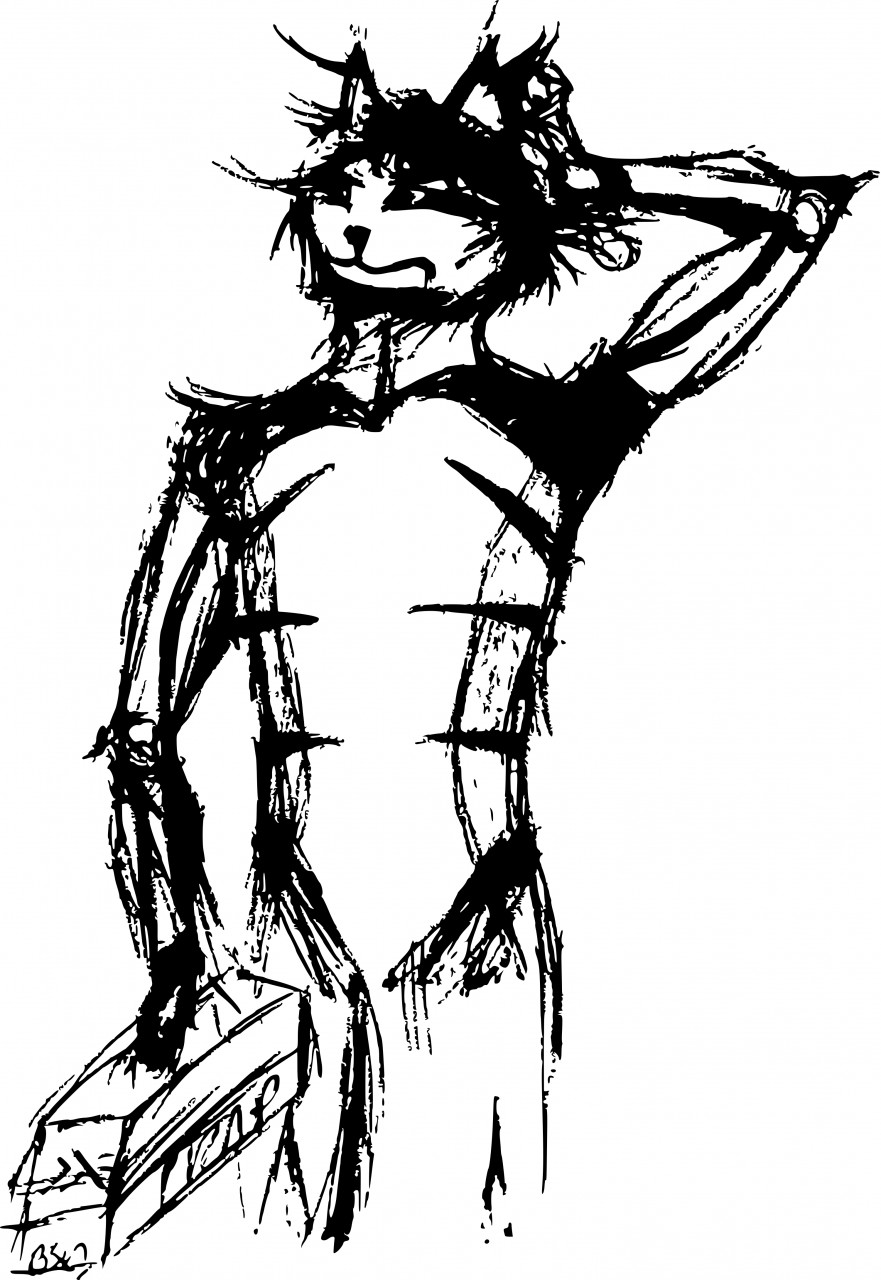
\includegraphics[keepaspectratio, width=\textwidth, height=0.75\textheight]{50x/toolbox/s1v1.jpg}
	\caption[center]{le pamoi versiio be la'oi .WESTERNUNIONSOFTHECOUNTRYWESTERNS.}
\end{figure}
\subsection{le remoi tsautu}
ni'o le remoi tsautu be la'oi.\ WESTERNUNIONSOFTHECOUNTRYWESTERNS.\ cu pamoi lo'i milxe xamgu pinsi bo tsautu\sds  .i ku'i ti poi tsautu cu .uaigri le vektori pixra poi kibzva la'o gy.\ \url{https://github.com/varikvalefor/drawingstuff/blob/master/50x/toolbox/toolboxsketch002.svg} .gy.

\begin{figure}[ht]
	\centering
	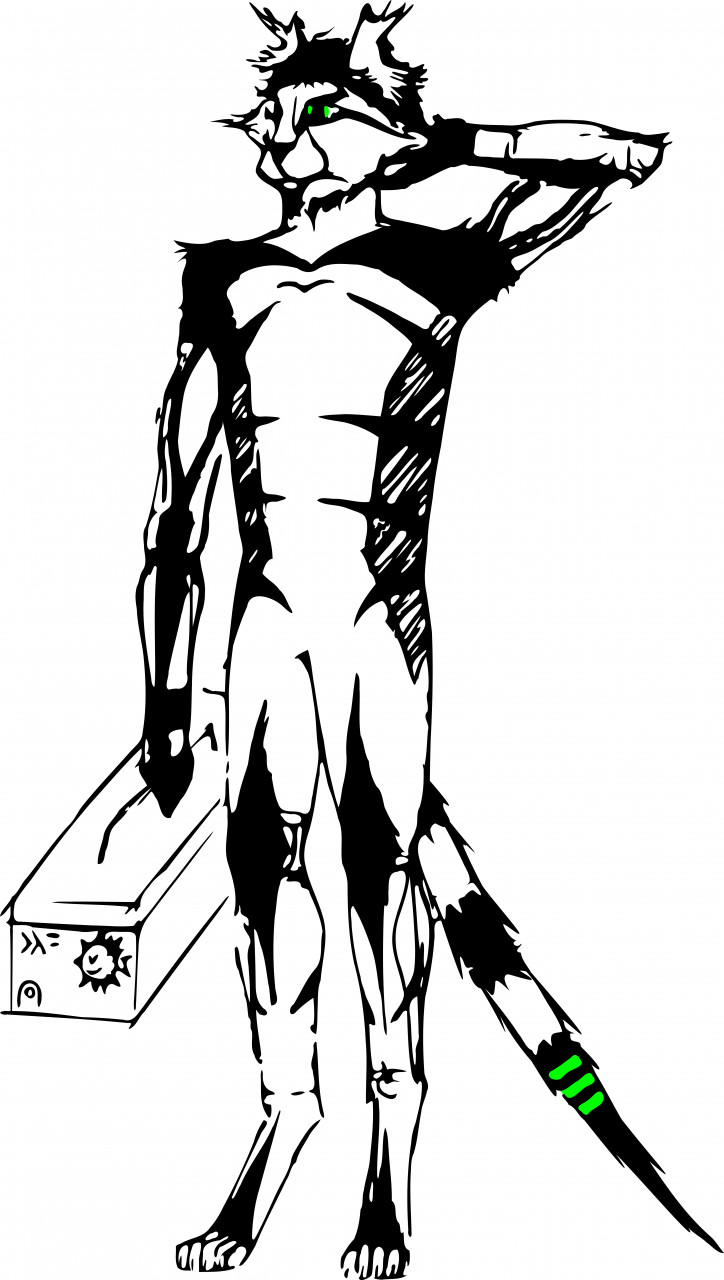
\includegraphics[keepaspectratio, width=\textwidth, height=0.75\textheight]{50x/toolbox/s1v2.jpg}
	\caption[center]{le remoi tsautu be la'oi .WESTERNUNIONSOFTHECOUNTRYWESTERNS.}
\end{figure}
\chapter{la'oi .HOLLYWOODFREAKSONTHEHOLLYWOODSCENE.}
\begin{figure}[ht]
	\centering
	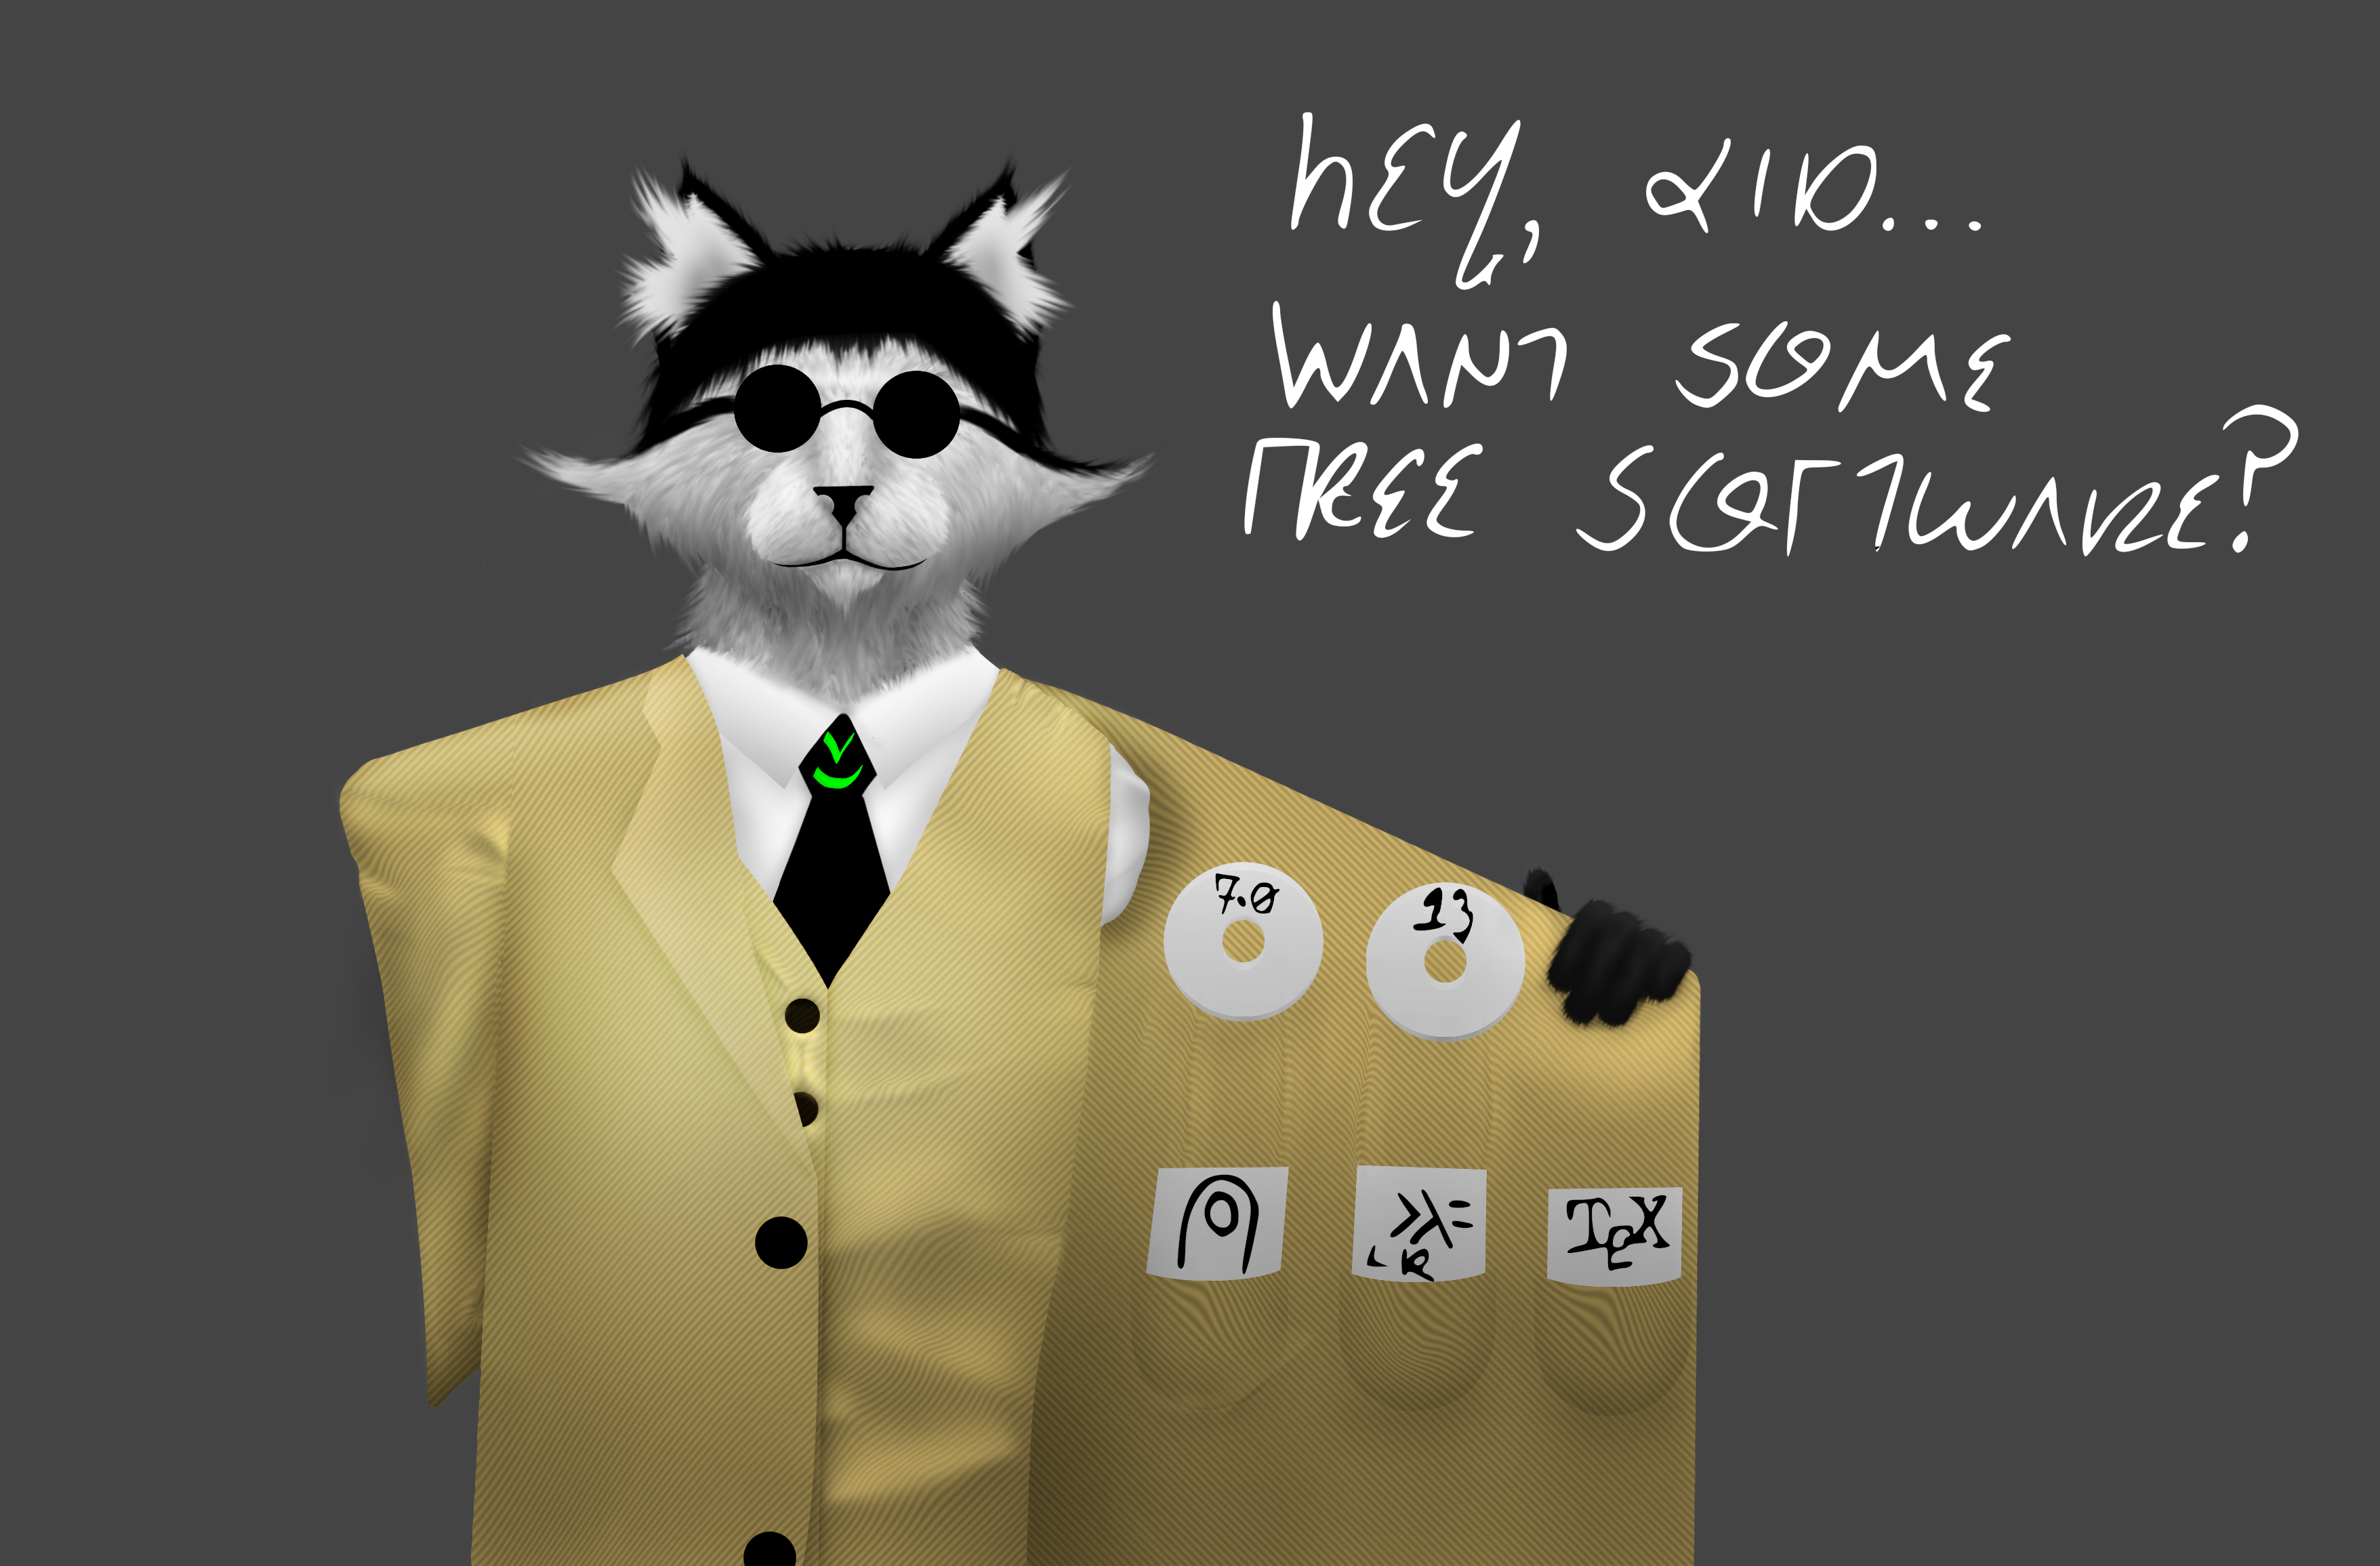
\includegraphics[keepaspectratio, width=\textwidth, height=0.75\textheight]{hollywoodfreaksonthehollywoodscene/hollywoodfreaksonthehollywoodscene.png}
	\caption[center]{la'oi .HOLLYWOODFREAKSONTHEHOLLYWOODSCENE.}
\end{figure}
\section{le pamoi velski be le pixra}
\subsection{le bebna ba'e tordu lisri}
ni'o le ctemidju cu tcika le nu lo prenu goi ko'a cadzu lo klaji\sds  .ije ko'a jibni lo dikca fatri dinju\sds  .ije le prenu poi se viska lo tcidu ku'o goi ko'e klama ko'a lo cmatricu

.i ko'a simlu le ka selspaji\sds  .ije ko'e cusku lu doi le verba\sds  .i xu do djica lo fingubni proga li'u

.i le tcidu cu kakne le nu jivbi'o lo jei fitytu'i

\subsection{la'oi .Blah.}
ni'o gubgau le bebna se xamsku

ni'o le pixra cu bebna se xamsku\sds  .i le nu la .varik.\ cu terxra cu pamoi jetnu ju'anai lo'i nu la .varik.\ cu terxra lo bukpu

\subsection{le selvau be le daski}
ni'o le se tcita be zoi gy.\ 7.0 .gy.\ be'o fa'u le se tcita be zo'oi .13.\ cu cukmirvelvei la'oi .OpenBSD.\ fa'u la'oi .FreeBSD.

\subsubsection{le cuktermai}
ni'o la .varik.\ cu djica le nu le pixra cu sitna le ziljmina proga kei ca'o le nu la .varik.\ cu zbasu fo'a\sds  .i da poi sidbo zo'u da na temsepcau mulno pe'a

\subsubsection{le kosta daski}
ni'o le tcidu cu sruma le du'u le daski cu vasru le papri poi krati pe'a lo te samrkompli po le sambau poi se pilno la .varik.

\subsubsection{li ni'e ni co'e}
ni'o la .varik.\ cu djica le nu le pixra cu sitna le ziljmina proga kei ca le nu la .varik.\ cu zbasu fo'a\sds  .i ku'i da poi sidbo zo'u da na temsepcau mulno pe'a

\subsection{lo cfilyfacki}
ni'o lo nu cfilyfacki cu roroi zanvi'e

\subsection{le pilno}
ni'o pilno la'oi .GIMP.\ le nu zbasu le pixra

ni'o pilno la'o gy.\ ed(1) .gy.\ le nu ciska dei

\section{le cfila be le pixra}
ni'o le su'o prenu poi ke'a na du la .varik.\ cu facki le du'u le taxfu poi ke'a se pixra la'oi .HOLLYWOODFREAKSONTHEHOLLYWOODSCENE.\ goi ko'a cu smimlu lo pelji

ni'o si'a la .varik.\ cu facki le du'u le cukmirvelvei poi ke'a se pixra ko'a cu smimlu lo pelji

\subsection{le taxfu poi ke'a claxu le ci cimde pe'a}
ni'o lo so'o prenu cu xusra le du'u le taxfu be la'oi .VUNC.\ ku'o poi ke'a se vasru la'oi .HOLLYWOODFREAKSONTHEHOLLYWOODSCENE.\ cu claxu le ci cimde pe'a je cu smimlu lo pelji ja zo'e

.i la .varik.\ cu tugni fi le xe famsku

.i fu'au le nu dasni lo veljmina be lo pelji kista je lo pelji nercreka je lo pelji creka vu'o poi ke'a claxu lo trixe cu mutce le ka ce'u xajmi

\subsection{le ctino po le cukmirvelvei}
.i la .varik.\ cu jinvi le du'u le velvei cu tamsmi lo pelji jenai lo cukmirvelvei\sds  .i cumki fa le nu le nabmi cu se rinka le ka le velvei cu tcenarkli

\chapter{la'oi .BROKEDOWNOUTINADITCHOFOLDRUBBISH.}
\begin{figure}[ht]
	\centering
	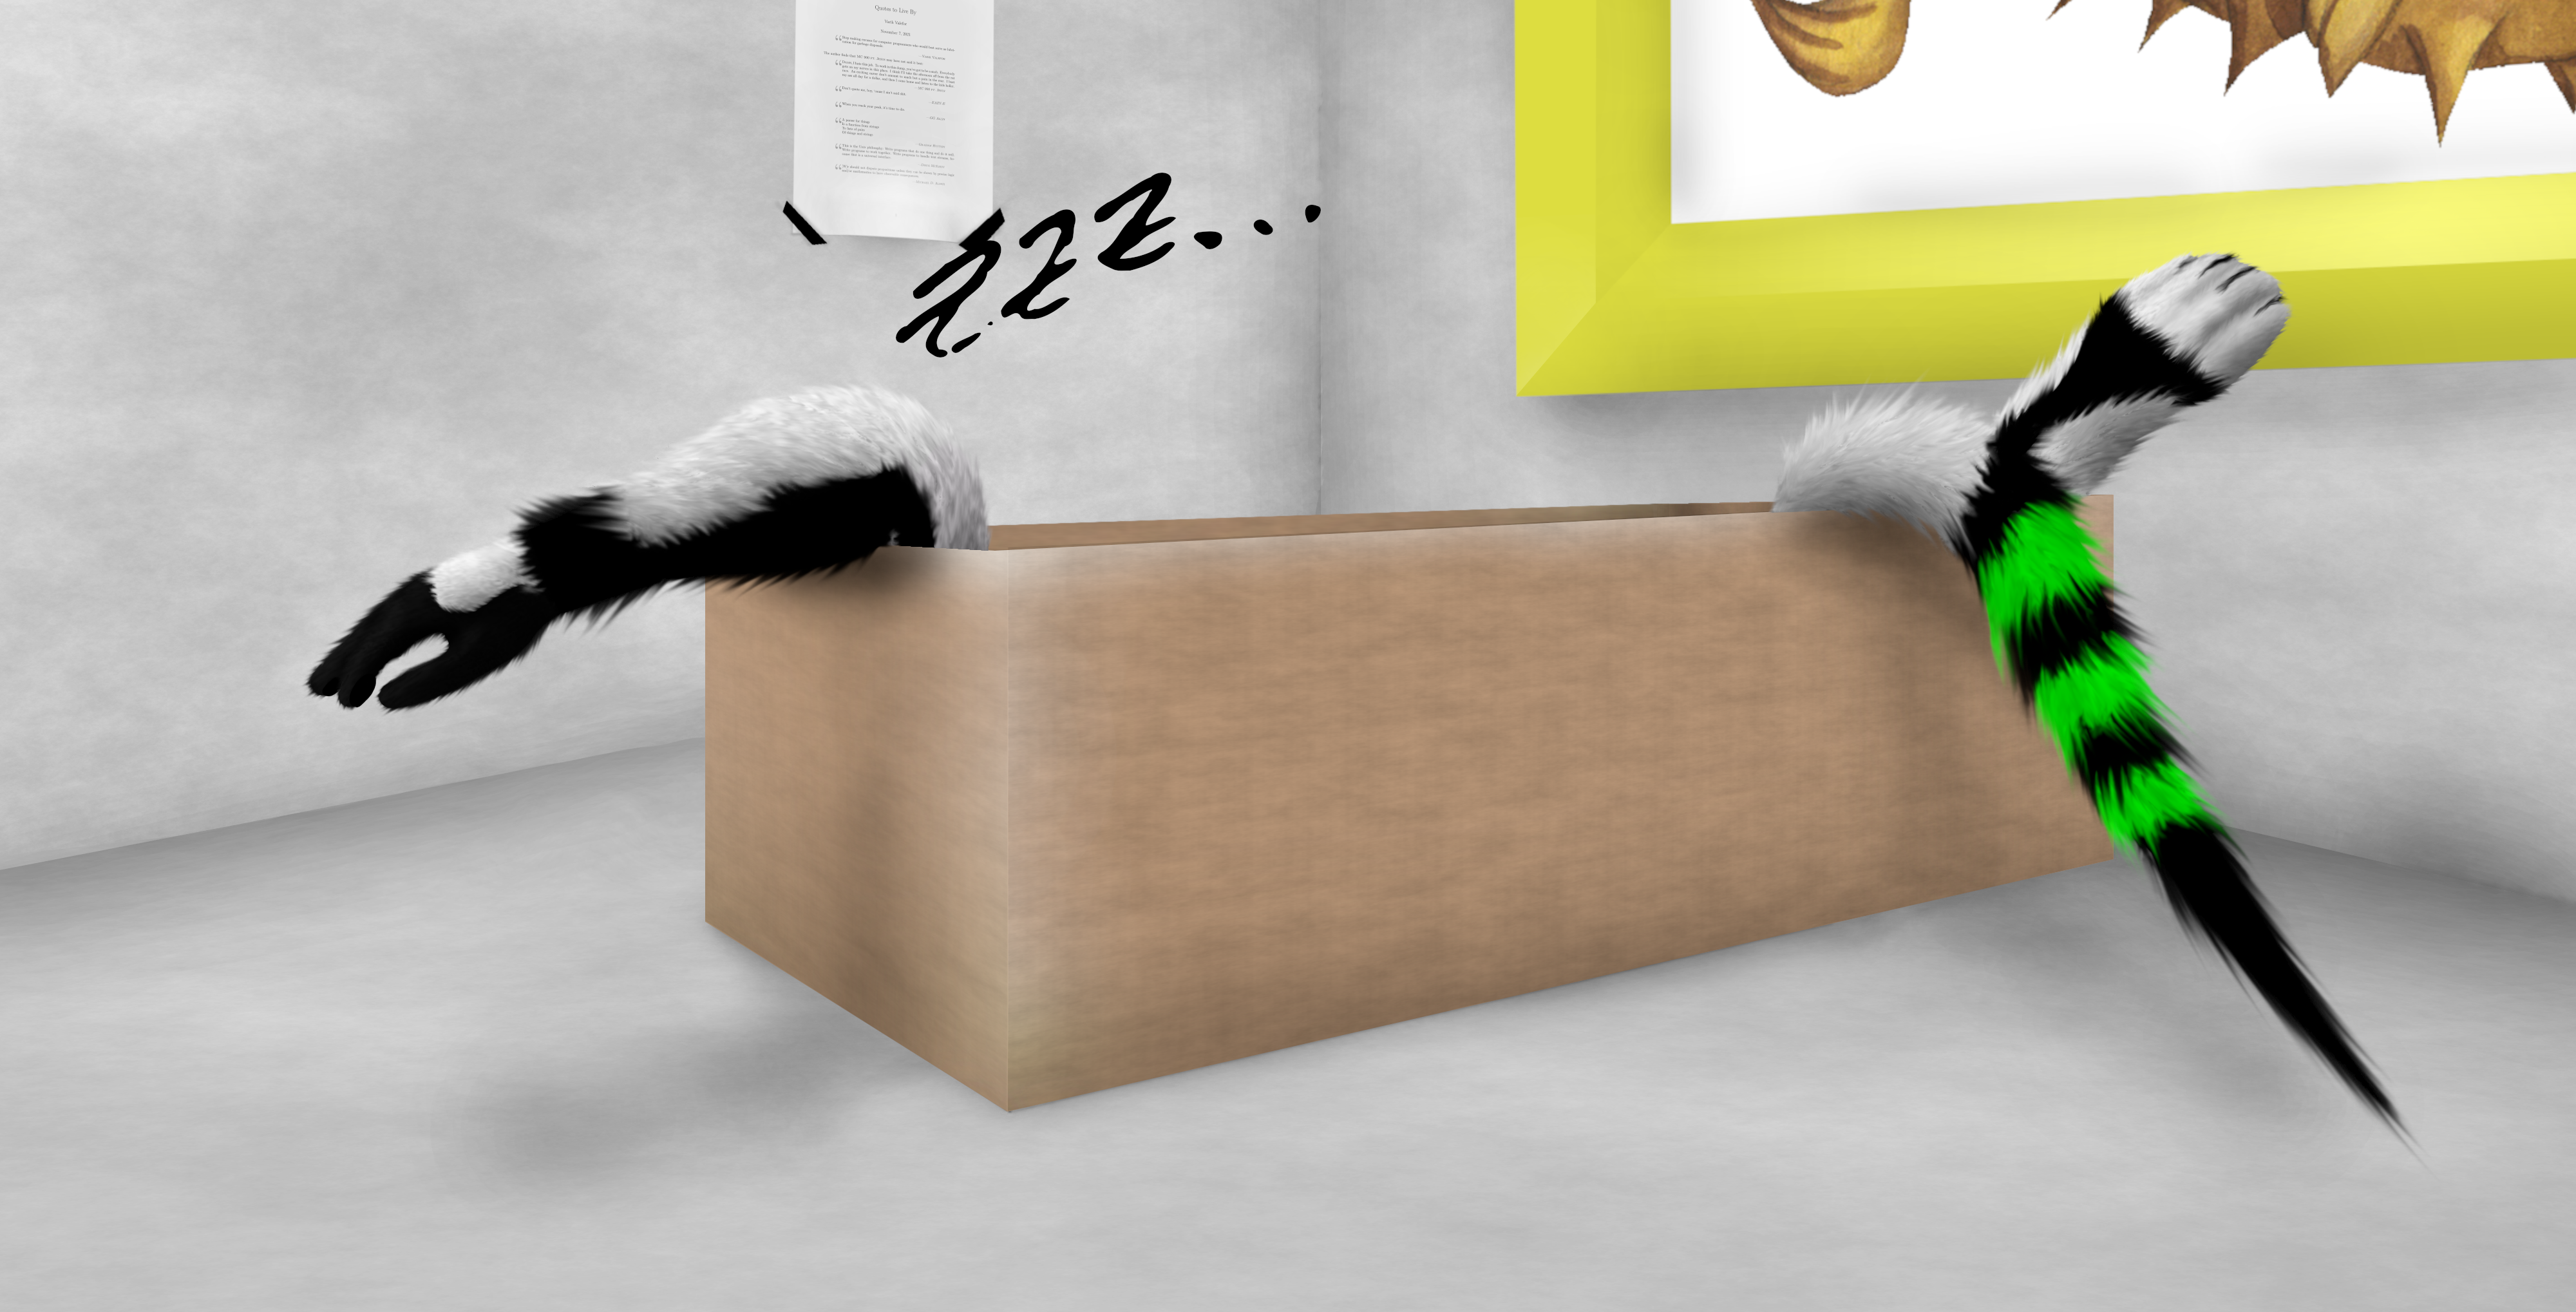
\includegraphics[width=\textwidth]{brokedownoutinaditchofoldrubbish/brokedownoutinaditchofoldrubbish.png}
	\caption[center]{.i le pixra cu du le pixra\sds  .i xu kanpe lo kacmyxra be lo snuji be loi xajre'u\sds  .i doi xlabebna ko na xlabebna}
\end{figure}
\section{le pamoi velski be le pixra}
ni'o lo cnino pixra cu gubni

\subsection{le jetnu pe'a trixe pixra\ldots je lo xamsku}
ni'o le pixra je cu se cmene zo'oi .BROKEDOWNOUTINADITCHOFOLDRUBBISH.\ cu pamoi lo gubni pixra be fi la .varik.\ ku poi ckaji lo jetnu pe'a trixe pixra je no lo stodi zilska je no lo sucta\sds  .i ji'a zo'oi .BROKEDOWNOUTINADITCHOFOLDRUBBISH.\ vasru lo so'u xamsku

\subsection{le tanxe}
ni'o cumki fa lo nu lo tcidu cu sruma le du'u le tinsypleta'e poi vasru le xarpre poi zutse cu se tsagau je cu na se marxa lo cmalu junta\sds  .i ji'a le tcidu cu cumki sruma le du'u le vorme pe'a po le tanxe cu se vasru le tanxe ja cu se vimcu

\subsection{lo se vasru pe'a xamsku}
ni'o le pamoi versiio be le pixra cu se vasru pe'a xamsku\sds  .i ciska le se vasru pe'a xamsku le tanxe\sds  .i ku'i la .varik.\ cu pu .uaigri jivbi'o le du'u le se vasru pe'a xamsku cu na mutce le ka xajmi kei kei je cu vimcu le se vasru pe'a xamsku

\subsection{zo'oi.\ ZZZ.}
ni'o le nu zo'oi .ZZZ.\ se pixra cu  .indika le du'u le xarpre cu sipsavgau\sds  .i le nu le xarpre cu sipsavgau kei  .indika le du'u le xarpre sipna\sds  .i ku'i zo'oi .ZZZ.\ kampu sipsav bo krati ki'u ma

\subsection{lo nu nitpiki}
ni'o lo nu nitpiki cu za'o se nelci

\subsection{le se cuxna xarci pe'a}
ni'o pilno la'oi .GIMP.\ le nu zbasu le pixra\sds  .i pilno lo xance degji .ualdo le jetnu pe'a pixra bo gunka

ni'o pilno la'o gy.\ ed(1) .gy.\ le nu ciska dei

ni'o la'oi .GIMP.\ je la'o gy.\ ed(1) .gy.\ bajra pe'a la'oi .OpenBSD.

\section{le cfila be le pixra}
ni'o selji'i fi ko'a goi la'oi .BROKEDOWNOUTINADITCHOFOLDRUBBISH.\ fa\ldots
\begin{itemize}
	\item le du'u ko'a toldra pixra\ldots
	\begin{itemize}
		\item le jamfu be la'oi .VUNC.\ be'o je
		\item le tanxe kei
	\end{itemize}
\end{itemize}
vu'o po'o nai

\subsection{le se cfifa'i be la .varik.}
ni'o la .varik.\ cu jinvi\ldots
\begin{itemize}
	\item le du'u ko'a goi la'oi .BROKEDOWNOUTINADITCHOFOLDRUBBISH.\ cu toldra pixra\ldots
	\begin{itemize}
		\item le jamfu be la'oi .VUNC.\ be'o je
		\item le tanxe kei
	\end{itemize}
\end{itemize}
vu'o po'o nai

\subsubsection{le ka ce'u xlali pixra le jamfu be la'oi .VUNC.}
ni'o la .varik.\ cu jinvi le du'u ko'a goi la'oi .BROKEDOWNOUTINADITCHOFOLDRUBBISH.\ cu toldra pixra le jamfu be la'oi .VUNC.\ kei ki'u le nu la .varik.\ cu jinvi le du'u ko'a pixra le nu le jmadegji be la'oi .VUNC.\ cu dukse le ka ce'u sampu je me'oi .rectangular.

\subsubsection{le ka ce'u xlali pixra le tanxe}
ni'o la .varik.\ cu jinvi le du'u ko'a goi la'oi .BROKEDOWNOUTINADITCHOFOLDRUBBISH.\ cu toldra pixra le tanxe poi ke'a vasru la'oi .VUNC.\ kei ki'u le nu la .varik.\ cu jinvi le du'u ko'a pixra le nu le darno je mlapau be le tanxe cu mleca le jibni je mlapau be le tanxe le ni ganra

\chapter{la'oi .DANCINGONTHEROOFSHOOTINGHOLESINTHEMOON.}
\begin{figure}[ht]
	\centering
	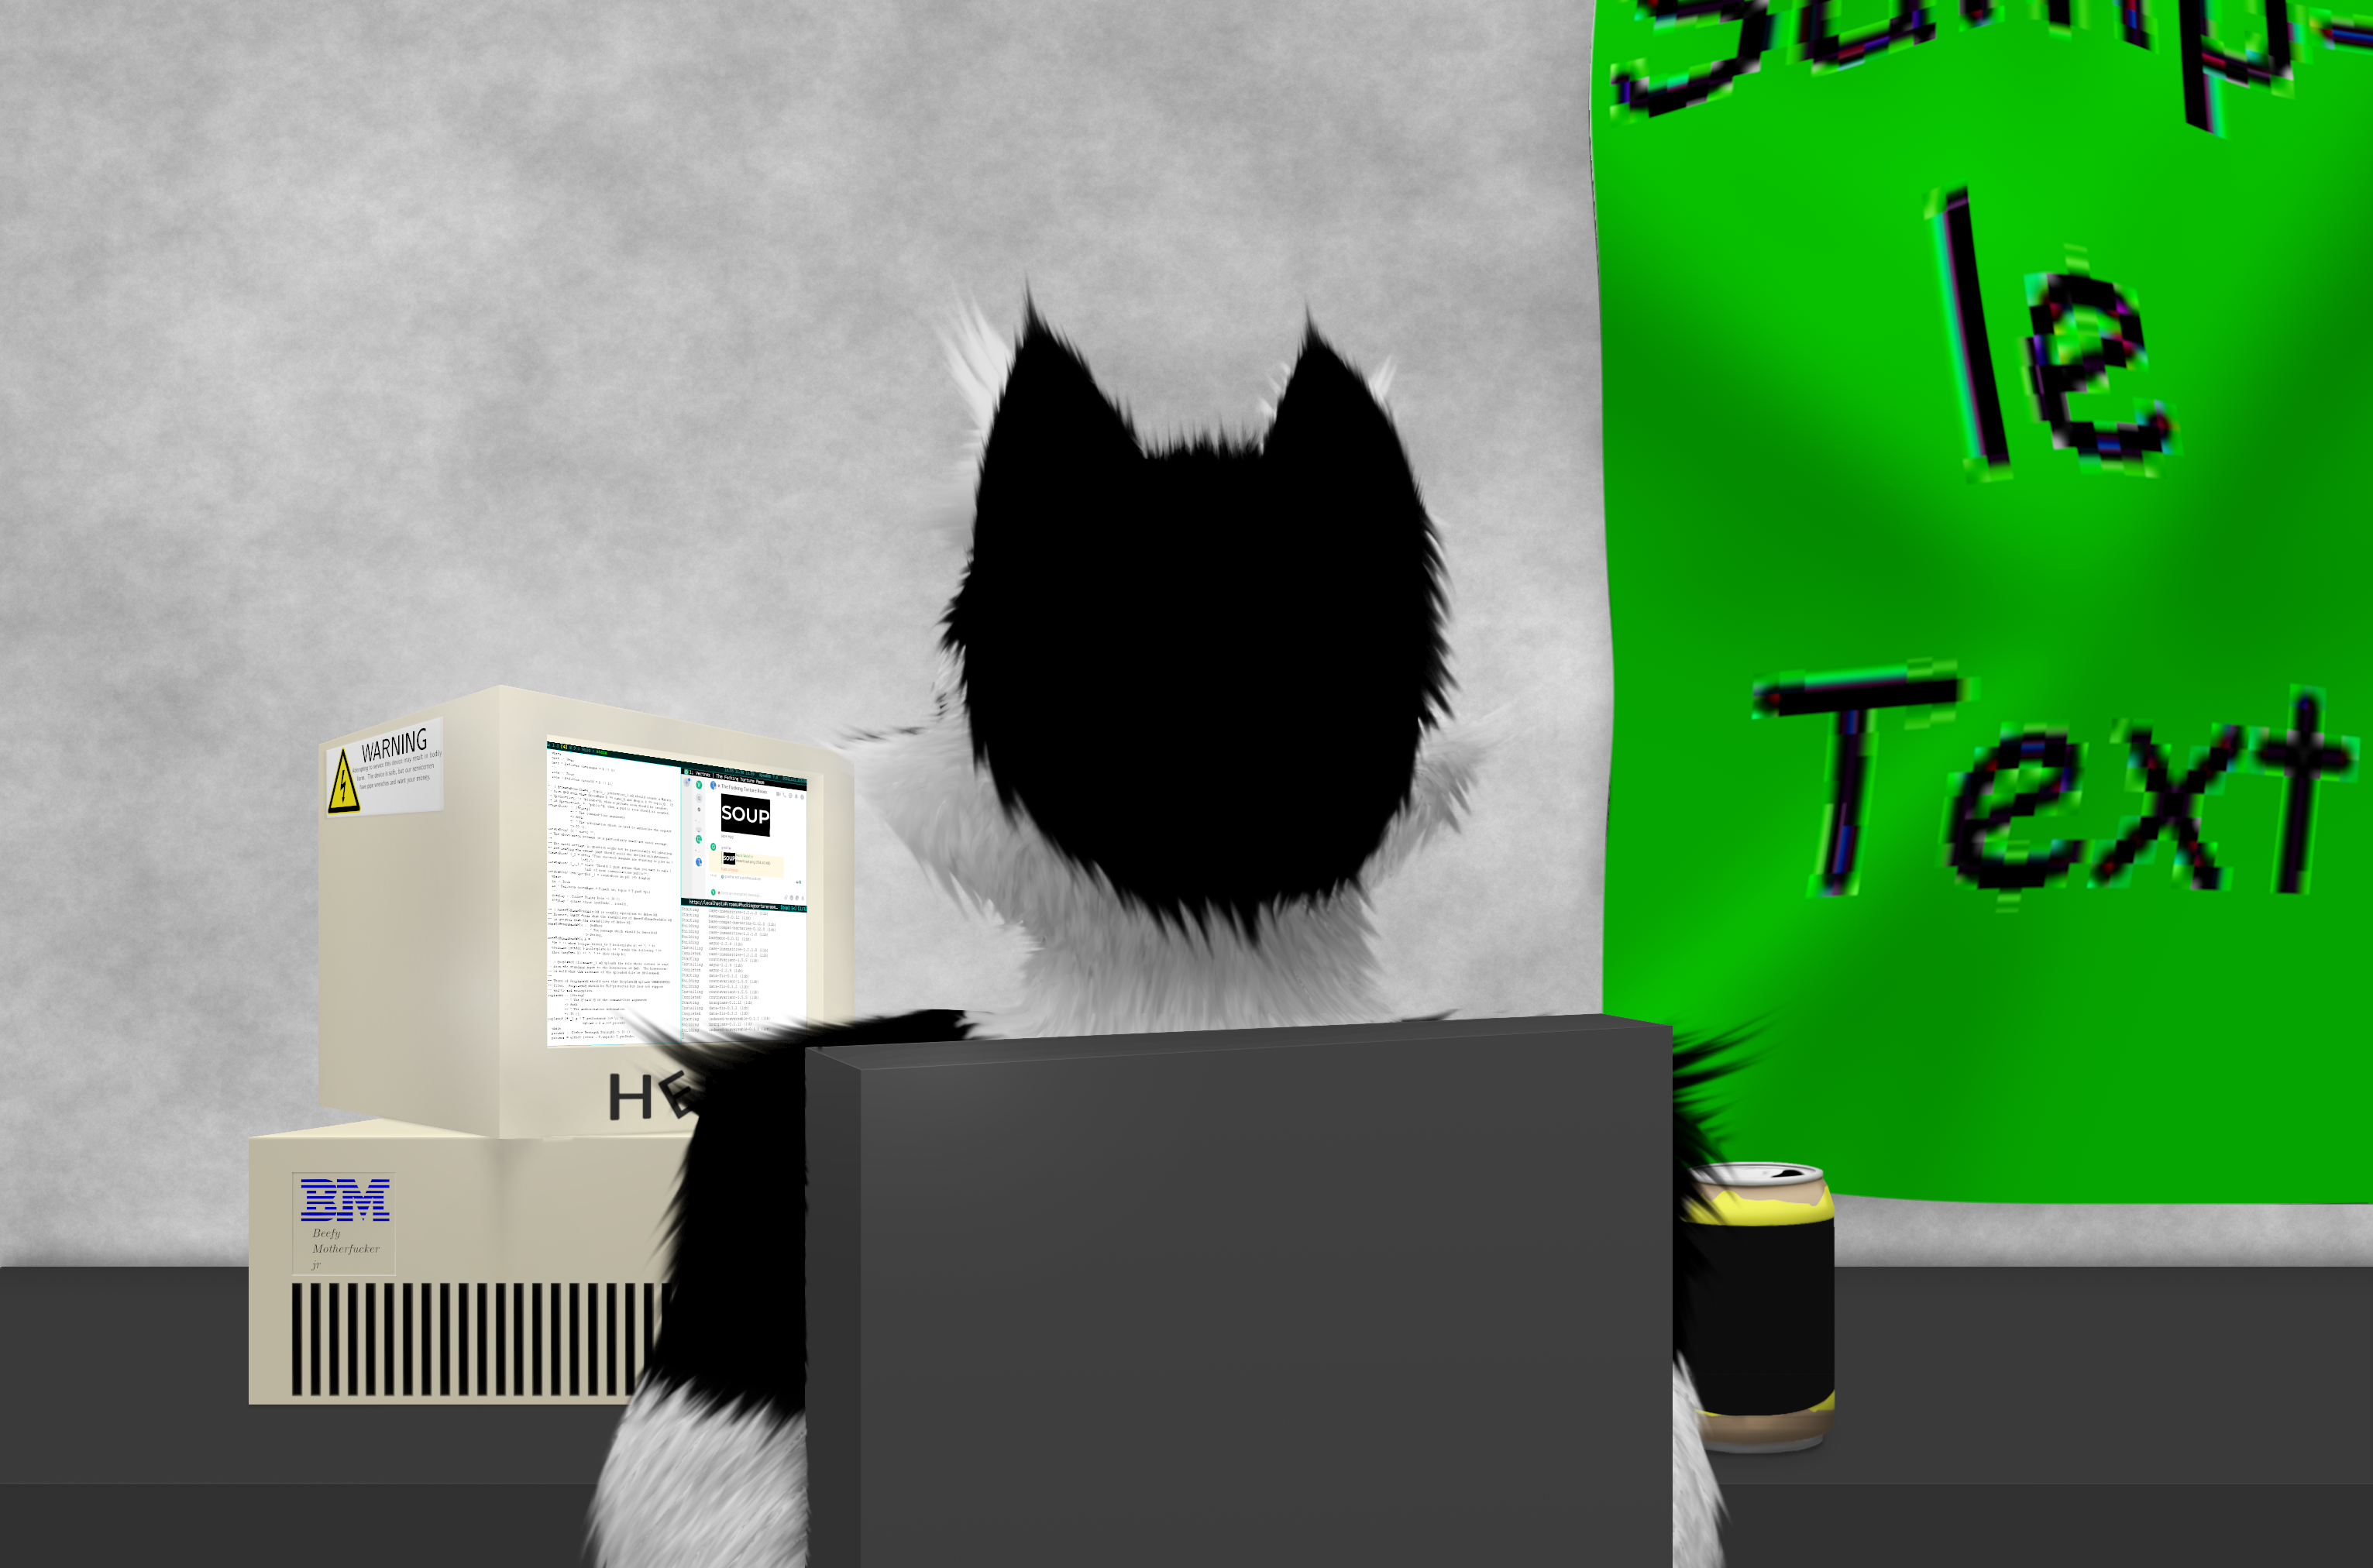
\includegraphics[width=\textwidth]{dancingontheroofshootingholesinthemoon/dancingontheroofshootingholesinthemoon.png}
	\caption[center]{ni'o le mulbi'o versiio be la'oi .DANCINGONTHEROOFSHOOTINGHOLESONTHEMOON.\sds  ni'o le nu viska lo ro tcila cu frili zo'e le nu pilno lo banro blaci\ldots ja lo cmactatci}
\end{figure}
\section{le pamoi velski be le pixra}
ni'o .ue'i lo ziljmina pixra cu gubni

ni'o le pixra cu pixra lo roldje tcini\sds  .i ku'i sorpa'a le nu le pixra cu na mutce le ka tolzdi

\subsection{le vlavelski}
zo'oi .VUNC.\ krati le xarpre be la .varik.
\subsection{le torveki}
ni'o le pixra cu pixra le nu la'oi .VUNC.\ jibni je cu galfi lo proga\ldots je cu tcidu lo xlali kibzva bo notci kei

\subsection{le se xamsku je zo'e}
ni'o le pixra cu simsa le da'a pixra be fi la .varik.\ li ni'e ni se vasru lo se xamsku\sds  .i le tcidu cumki ciksi le xamsku\sds  .i ku'i ji'a le pixra cu vasru le cmalu jikske bo ckipinka\sds  .i ji'a le tcidu cu cumki skicu le cmalu jikske bo ckipinka

\subsection{zo'oi .SOUP.}
ni'o zo'oi .SOUP.\ poi simlu lo bebna cu zvati ki'u le nu la .varik.\ cu na djuno le du'u selfladra le nu le pixra cu zifre vasru le pamoi kacmyxra\sds  .i le nu na te nunflapai la .varik.\ cu frili la .varik.\ le nu le velski pe'a be le kacmyxra cu basti le pamoi kacmyxra

ni'o zo velski cu sidysmu ki'u le velski pe'a cu na mutce le ka skicu\sds  .i lo zenba velski velski be le pamoi kacmyxra cu du lo'u lo tcesedemri'a kacmyxra be lo kabri poi se vasru lo .alfabeta stasu le'u

\subsection{le kadje tcita}
ni'o le se tcidu po le kadje tcita cu du zoi gy.
\begin{quote}
	WARNING

	Attempting to service this device may result in bodily harm.  The device is safe, but our servicemen have pipe wrenches and want your money.
\end{quote}
.gy.

\subsection{le batkyfoi}
ni'o le pixra cu pixra le nu la'oi .VUNC.\ pilno le batkyfoi\sds  .i ku'i le batkyfoi naseviska\sds  .i ku'i je se cumki le nu le du'u la'oi .VUNC.\ pilno le batkyfoi kei zenba xamgu se  .indika

\subsection{le nu nitpiki}
ni'o lo nu nitpiki cu za'o se nelci

\subsection{le plijaspu}
ni'o le pixra cu selxrapra je cu selplijaspu la'o gy.\ CC BY-NC 4.0 .gy.\sds  .i le mulno tcidu po ti poi selplijaspu cu xabju pe'a la'o gy.\ \url{https://creativecommons.org/licenses/by-nc/4.0/legalcode} .gy.

\subsection{le pilno}
ni'o pilno la'oi .GIMP.\ le nu zbasu le pixra\sds  .i la'oi .GIMP.\ tcexla\sds  .i ku'i za'a la'oi .GIMP.\ traji le ka ce'u xamgu pixra bo fingubni bo proga

ni'o pilno la'o gy.\ ed(1) .gy.\ le nu zbasu dei

ni'o la'oi .GIMP.\ je la'o gy.\ ed(1) .gy.\ bajra pe'a la'oi .OpenBSD.

\section{le selji'i be fi le pixra}
ni'o le stizu poi ke'a selzutse la'oi .VUNC.\ cu claxu lo tcila

\subsection{le stizu}
ni'o le nu le stizu poi selzutse la'oi .VUNC.\ cu claxu lo tcila cu se rinka le nu le stizu tengu cu .ambigu'o\sds  .i le stizu se .enge cu se staile\sds  .i la .varik.\ cu mutce le ka nelci lo dijyzbaske po la'oi .Brutalism.\sds  .i ku'i krici le du'u le stizu cu mabla

\chapter{la'oi .ITHINKWEREGOINGCRAZY.}
\begin{figure}[ht]
	\centering
	\includegraphics[width=10cm]{ithinkweregoingcrazy/ithinkweregoingcrazy.png}
	\caption[center]{la'oi .ITHINKWEREGOINGCRAZY.}
\end{figure}
\section{le pamoi skicu be le pixra}
ni'o zoi gy.\ BLOCKED BY SHODAN LEVEL SECURITY .gy.

\subsection{lu mi viska ma li'u}
ni'o le pixra cu pixra le nu le xarpre be la .varik.\ cu smimlu la'oi .SHODAN.\ po la'o gy.\ \textit{System Shock} .gy.\ le ka jorne lo jimsko kei je le ka selnunfirsku fi lo nutli

\subsection{le tcika}
ni'o ji'i za'a le pavrelmasti cu vasru pe'a lo su'o pa pixra

\subsection{le citri}
\subsubsection{le tsautu}
ni'o lo pamuki'oki'o nanca cu se puvza le nu la .varik.\ cu gubni le tsautu poi pixra le nu la'oi .VUNC.\ simlu la'oi .SHODAN.\ po la'o gy.\ \textit{System Shock} .gy.\ le ke jorne lo jimsko

\subsubsection{le pamoi se troci se galfi}
ni'o la .varik.\ cu tolsti le nu galfi le tsautu lo jetnu pe'a pixra\sds  .i ku'i le nu la .varik.\ cu zbasu lo nurfu'i cu se purci snuti vimcu le datni be le cukmakyvelvei po le ralju skami po la .varik.\sds  .i ja'e lakne fa le pamoi versiio be le pixra cu cimni bo farcri pe'a

\subsubsection{le remoi se troci se galfi}
ni'o li papa pi'e vo pi'e renorepa cu detri le nu la .varik.\ cu tolsti le nu galfi le tsautu lo jetnu pe'a pixra je cu jmina lo tsautu poi nasevasru loi sirsunla lo samrxra be fi la'o gy.\ Scalable Vector Graphics .gy.\sds  .i snada le nu mulno le pruce

\subsubsection{le nu troci le nu jmina lo tcila}
ni'o li ji'i re pi'e xa pi'e renorepa cu detri le nu la .varik.\ cu galfi le samrxra be fi la'o gy.\ Scalable Vector Graphics .gy.\ lo samrxra be fi la'oi .XCF.\ je cu tolsti le nu jmina lo tcila\sds  .i le nu jmina lo tcila cu lidne le nu jmina lo jimsko kei ki'u zo'e

ni'o lo jetnu pe'a nabmi ku sotmei\sds  .i ku'i la .varik.\ cu nanelci le jalge be le nu jmina le tcila kei je cu zasysti le nu zbasu le pixra

\subsubsection{le nu se snada jmina bo tcila}
ni'o li reze pi'e papa pi'e renorepa cu detki le nu la .varik.\ cu to'e zasysti le nu zbasu le pixra je ku'i cu ninke'u jivbi'o le du'u la'oi .GIMP.\ cumki kalci\ldots pe'a

\subsubsection{le nu mulgau le pixra}
ni'o li pa pi'e pare pi'e renorepa cu detni le nu la .varik.\ cu xusra le du'u le pixra cu selmulgau

\subsection{le nu le le pixra cu te gumgau}
ni'o ko'a goi la'oi .SHODAN.\ po la'o gy.\ \textit{System Shock} .gy.\ velfi'i le pagbu be le pixra ku poi se finti fo ko'a\sds  .i ku'i la .varik.\ cu napilno lo pa versiio be ko'a ca le nu la .varik.\ cu zbasu le pixra\sds  .i lo menli gumgau be ko'a po la'o gy.\ \textit{System Shock} .gy.\ je ko'a po la'o gy.\ \textit{System Shock 2} .gy.\ cu velfi'i le pixra ku'o fo la .varik.
\subsection{lo nu nitpiki}
ni'o lo nu nitpiki cu za'o se nelci

\subsection{le plijaspu}
ni'o le pixra cu selxrapra je cu selplijaspu la'o gy.\ CC BY-NC 4.0 .gy.\sds  .i le mulno tcidu po ti poi selplijaspu cu xabju pe'a la'o gy.\ \url{https://creativecommons.org/licenses/by-nc/4.0/legalcode} .gy.

\subsection{le pilno}
ni'o pilno la'oi .GIMP.\ le nu majgau le pixra\sds  .i  la'oi .GIMP.\ xlatce\sds  .i ku'i zmanei la'oi .GIMP.\ la'oi .Krita.

ni'o ciska dei fo la'o gy.\ ed(1) .gy.

ni'o la'oi .GIMP.\ je la'o gy.\ ed(1) .gy.\ bajra pe'a la'oi .OpenBSD.

\section{le kanla se cortu}
ni'o so'u da poi prenu zo'u da xusra le du'u le nu da catlu la'o .ITHINKWEREGOINGCRAZY.\ cu se jalge le nu da cortu kei kei goi ko'a\sds  .i la .varik.\ cu jijyji'i le du'u lo prenu poi xusra ko'a cu du'eski ko'a ja cu bilma lo kanla se cortu kei ki'u le nu la .varik.\ cu na zatfa'i lo satci krasi be le kanla se cortu

\section{le se frati}
ni'o le nu la'oi .ITHINKWEREGOINGCRAZY.\ nasopnelsei\ldots cu cumki se krinu le nu zo'e poi velfi'i la'oi .ITHINKWEREGOINGCRAZY.\ rirci

\subsection{le velski be le se frati}
ni'o su'o da poi pixra fi la .varik.\ zo'u li ni'e ni lo prenu cu nelci la'oi .ITHINKWEREGOINGCRAZY.\ cu dubme'a li ni'e ni lo prenu cu nelci da

\subsection{le cumki rinka be le nu na selnei}
ni'o la .varik.\ cu jinvi le du'u le nu na nelci la'oi .ITHINKWEREGOINGCRAZY.\ cu cumki se krinu le nu zo'e poi velfi'i la'oi .ITHINKWEREGOINGCRAZY.\ rirci

\begin{thm}
ni'o lakne fa le du'u lo so'u prenu cu nelci la'oi .ITHINKWEREGOINGCRAZY.

\end{thm}

\begin{proof}
${}$

ni'o ro da zo'u ro de poi pixra zo'u ro di poi prenu zo'u le du'u de velsitsku da cu nibyti'i le du'u di mulsmujmi de na ja cu se slabu de

ni'o ro da poi pixra zo'u le du'u lo so'u prenu ku mulsmujmi da cu nibyti'i le du'u lakne fa le du'u lo so'u prenu ku nelci da\footnote{ni'o le tcidu cu se darsygau milxe bo senpi le pixra}

ni'o so'u prenu cu slabu la'o gy.\ \textit{System Shock} .gy.\footnote{ni'o cumki fa lo nu zo so'u dukse le ka ce'u ruble}

ni'o la'oi .ITHINKWEREGOINGCRAZY.\ velsitsku la'o gy.\ \textit{System Shock} .gy.

ni'o ja'e lakne fa le du'u lo so'u prenu cu nelci la'oi .ITHINKWEREGOINGCRAZY.
\end{proof}

\chapter{la'oi .JUDASTRAINWRECK.}
\begin{figure}[ht]
	\centering
	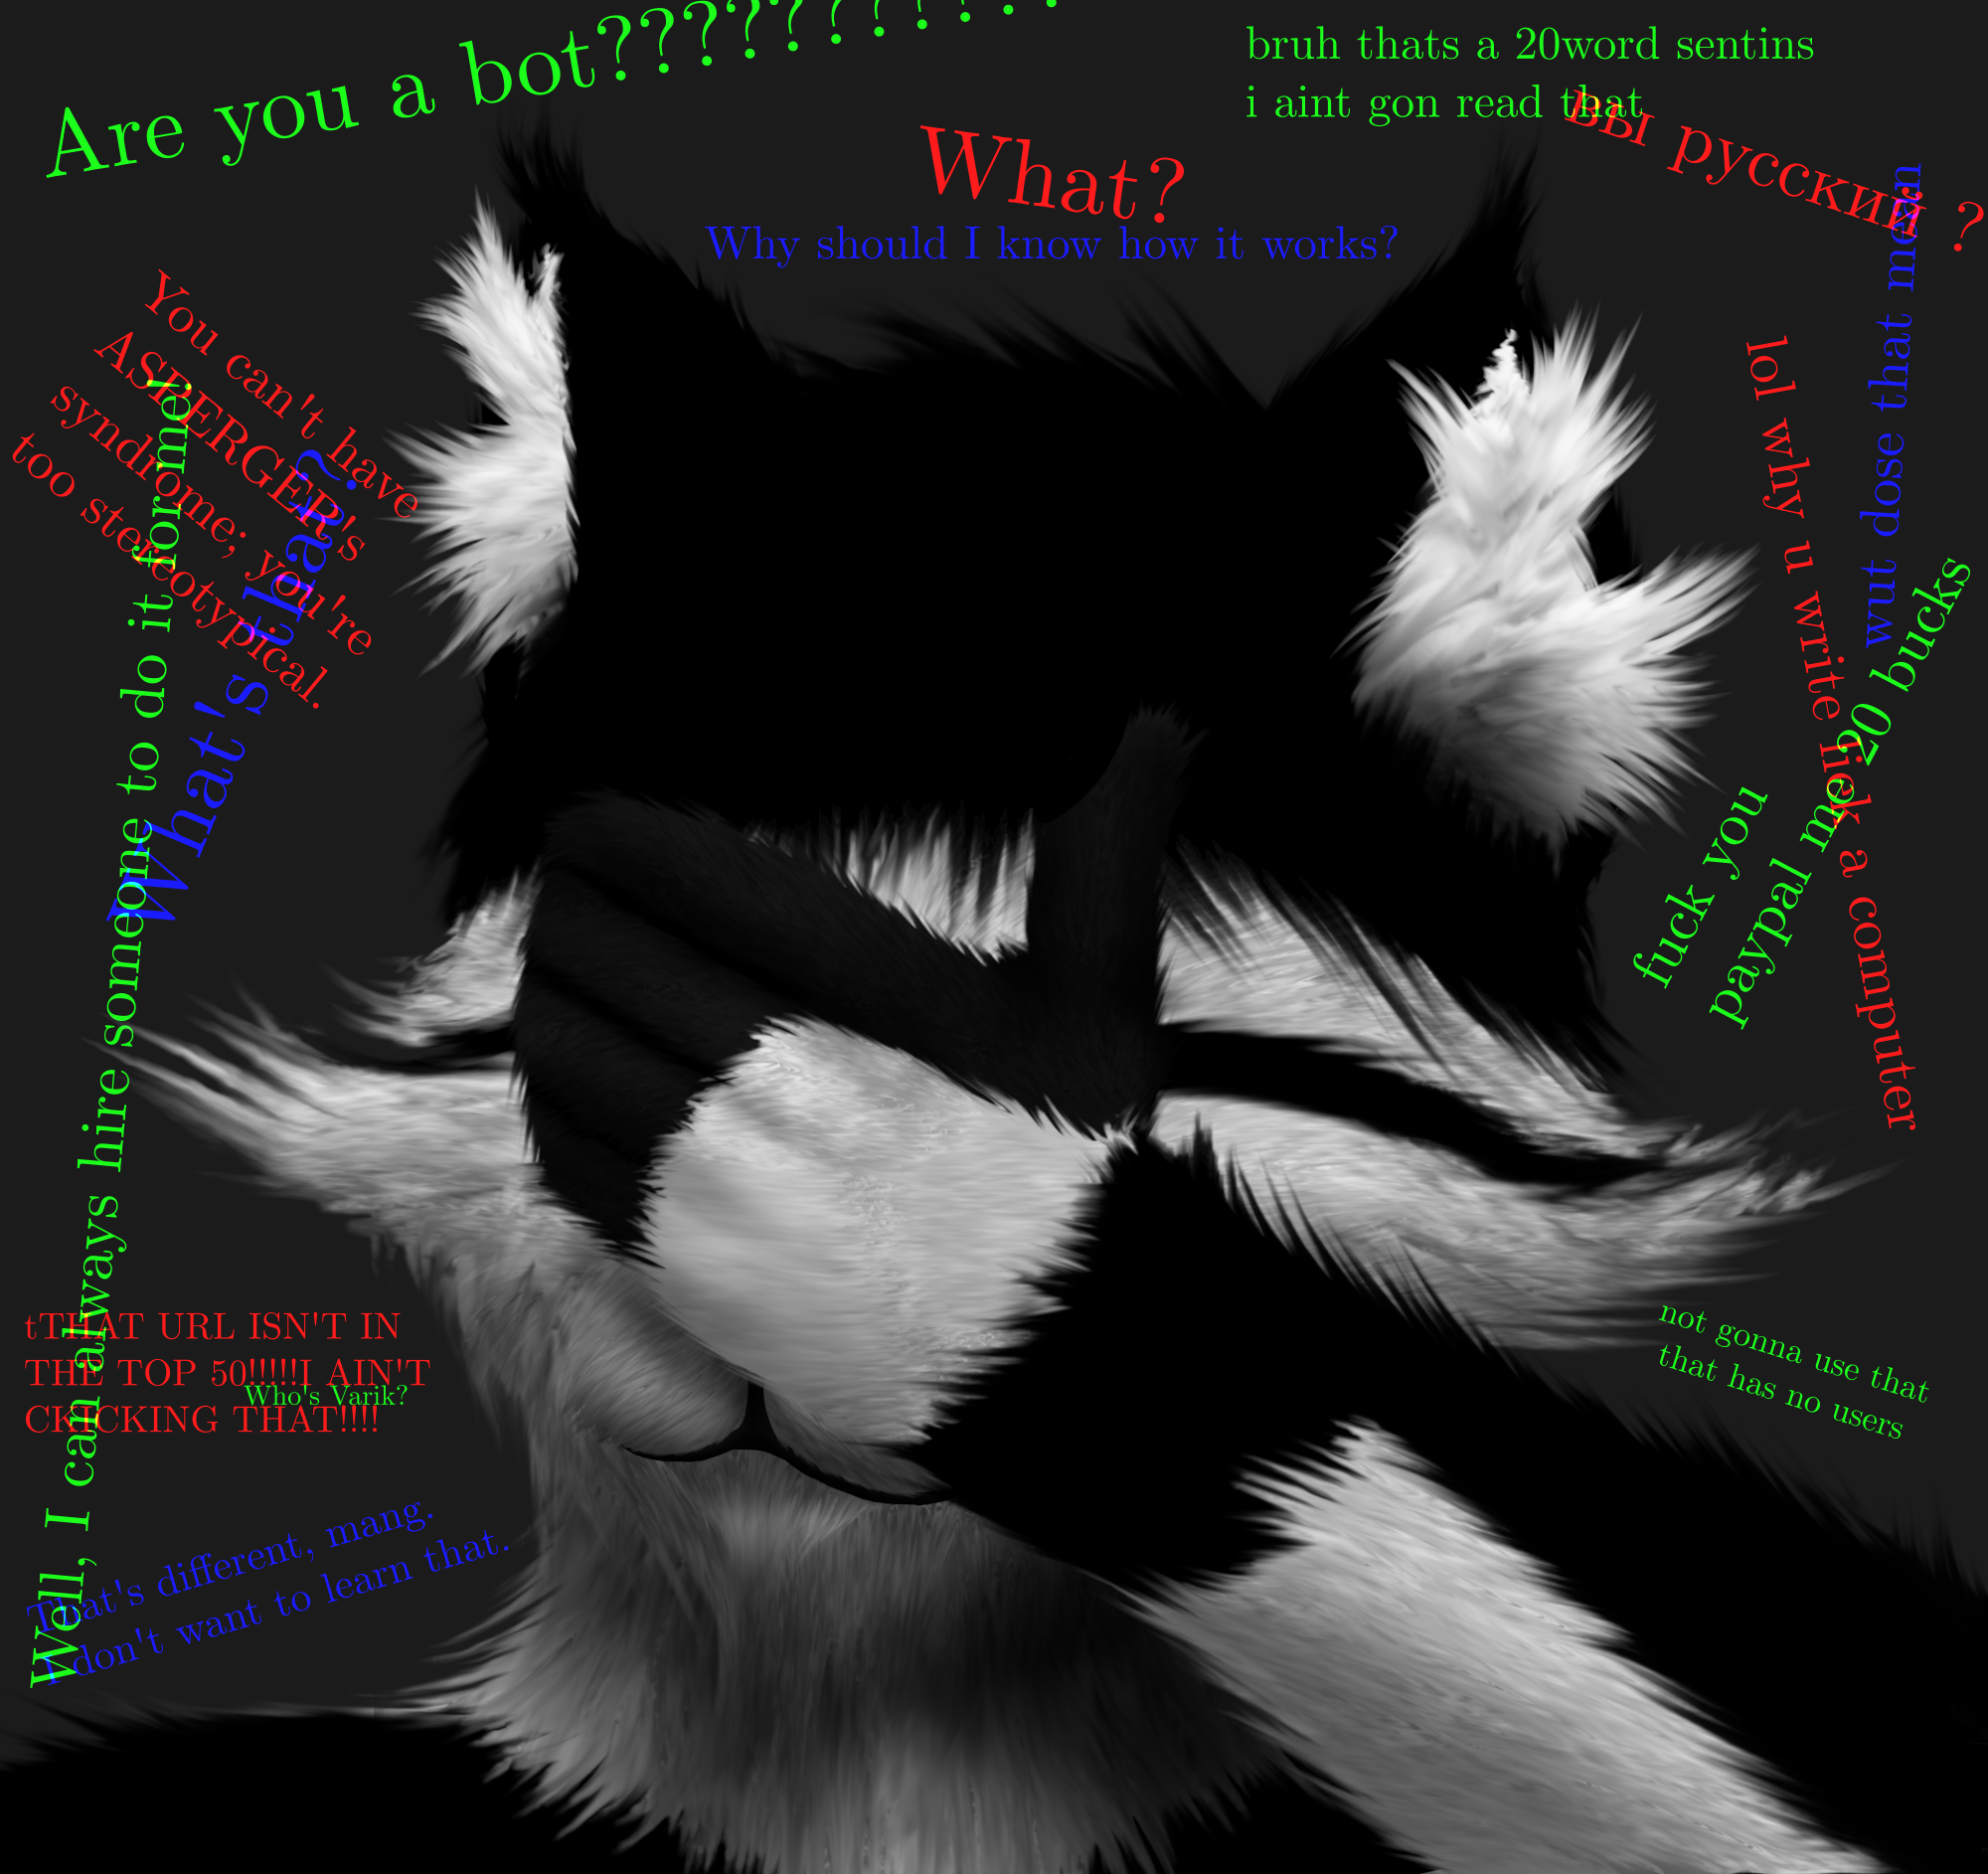
\includegraphics[width=10cm]{judastrainwreck/judastrainwreck.png}
	\caption[center]{la'oi .JUDASTRAINWRECK.}
\end{figure}
\section{le pamoi velski be le pixra}
ni'o la .varik.\ cu jinvi le du'u le firxa'e cu melbi

\subsection{le torveki}
ni'o su'o da poi papri bo pixra tsautu zo'u da binxo le vektori pixra poi binxo le pixra

ni'o le selci'a tanxe pe'a cu vasru lo toltce bo galfi notci poi pu selterbe'i la .varik.

ni'o le pixra cu selxrapra je cu selplijaspu la'o gy.\ CC BY-NC 4.0 .gy.

ni'o doi la'oi .lamer.\footnote{ni'o cumki fa lo nu lu lo me'oi .lamer.\ li'u cu zmadu lu la'oi .lamer.\ li'u le ka mapti\sds  .i ku'i .arxivo}\ ko pilno la'oi .OpenBSD.

\subsection{le pruce poi gasnu le nu le tsautu ku binxo le mulno pixra}
ni'o la .varik.\ cu majgau le pamoi tsautu ki'u le nu la .varik.\ cu djica le nu la .varik.\ cu terxra lo nasteci

.i la .varik.\ cu gasnu le nu le pamoi tsautu cu binxo le vektori pixra ki'u le nu la .varik.\ cu djica le nu la .varik.\ cu terxra lo trina

.i le nu la .varik.\ cu terxra le cabna pixra cu milxe se krinu le nu la .varik.\ cu djica le nu la .varik.\ cu ckasu lo prenu poi cusku lo bebna preti ja cu bebna pensi

\subsection{le selci'a tanxe pe'a}
ni'o le selci'a tanxe pe'a vasru lo toltce bo galfi notci poi pu selterbe'i la .varik.

.i la .varik.\ cu fuktra la'o gy.\ SIDESHOW BOB .gy.\ le nu cmoni kei ba le nu la .varik.\ cu jdice le du'u le nu la .varik.\ cu ckasu le prenu je cu curmi le nu le prenu ku cmecau cu filri'a le nu cmila

\subsection{le plijaspu}
ni'o le pixra cu selxrapra je cu selplijaspu la'o gy.\ CC BY-NC 4.0 .gy.\sds  .i le mulno tcidu po ti poi selplijaspu cu xabju pe'a la'o gy.\ \url{https://creativecommons.org/licenses/by-nc/4.0/legalcode} .gy.

\subsection{le pilno}
ni'o pilno la'oi .GIMP.\ le nu majgau le pixra\sds  .i  la'oi .GIMP.\ xlatce\sds  .i ku'i zmanei la'oi .GIMP.\ la'o gy.\ Krita  .gy.

ni'o ciska dei fo la'o gy.\ ed(1) .gy.

ni'o la'oi .GIMP.\ je la'o gy.\ ed(1) .gy.\ bajra pe'a la'oi .OpenBSD.

\section{le selji'i be fi la'oi .JUDASTRAINWRECK.}
ni'o selji'i fi la'oi .JUDASTRAINWRECK.\ goi ko'a fa\ldots
\begin{itemize}
	\item le du'u ko'a  .indika ko'e goi le du'u le selxra be ko'a cu mapra keitci kei ku ri'a le nu ko'a  .indika le du'u le kerfa be ko'e cu dukse kei kei kei noi te toltu'i fi la .varik.\ ku'o je
	\item le du'u ko'a pixra le .ambigu kei noi te mlitu'i fi la .varik.\ ku'o je
	\item le du'u ko'a citmle kei noi no'e te tugni fi la .varik.\ ku'o je
	\item le du'u ko'a pixra le nu le cmalu sirsunla bo tcila be le zunle molmla bo me'oi .tuft.\ be la'oi .VUNC.\ cu na mapti le barda sirsunla bo tcila be le zunle molmla bo me'oi .tuft.\ be la'oi .VUNC.\ kei kei noi ke'a te tugni fi la .varik.\ ku'o
vu'o po'o nai
\end{itemize}

\subsection{le ctino}
ni'o la .varik.\ cu jinvi le du'u cumki fa le nu ko'a goi la'oi .JUDASTRAINWRECK.\ dukse le ka ce'u vasru le ctino kei kei kei je le du'u ko'a dukse le ka ce'u manku

\subsection{le xance}
ni'o tu'a la'oi .JUDASTRAINWRECK.\  .indika le du'u ko'a goi le xandegji be fi la'oi .VUNC.\ cu tordu\sds  .i ku'i ko'a na tordu\sds  .i la'oi .JUDASTRAINWRECK.\ xlali pixra le xance be la'oi .VUNC.\sds  .i la'e di'u xajmi la .varik.

\section{le da'a versiio be le pixra}

\subsection{la'o pixrycmene.\ JUDASTRAINWRECK\hyp NOHANDLEBARS .pixrycmene.}
\begin{figure}[ht]
	\centering
	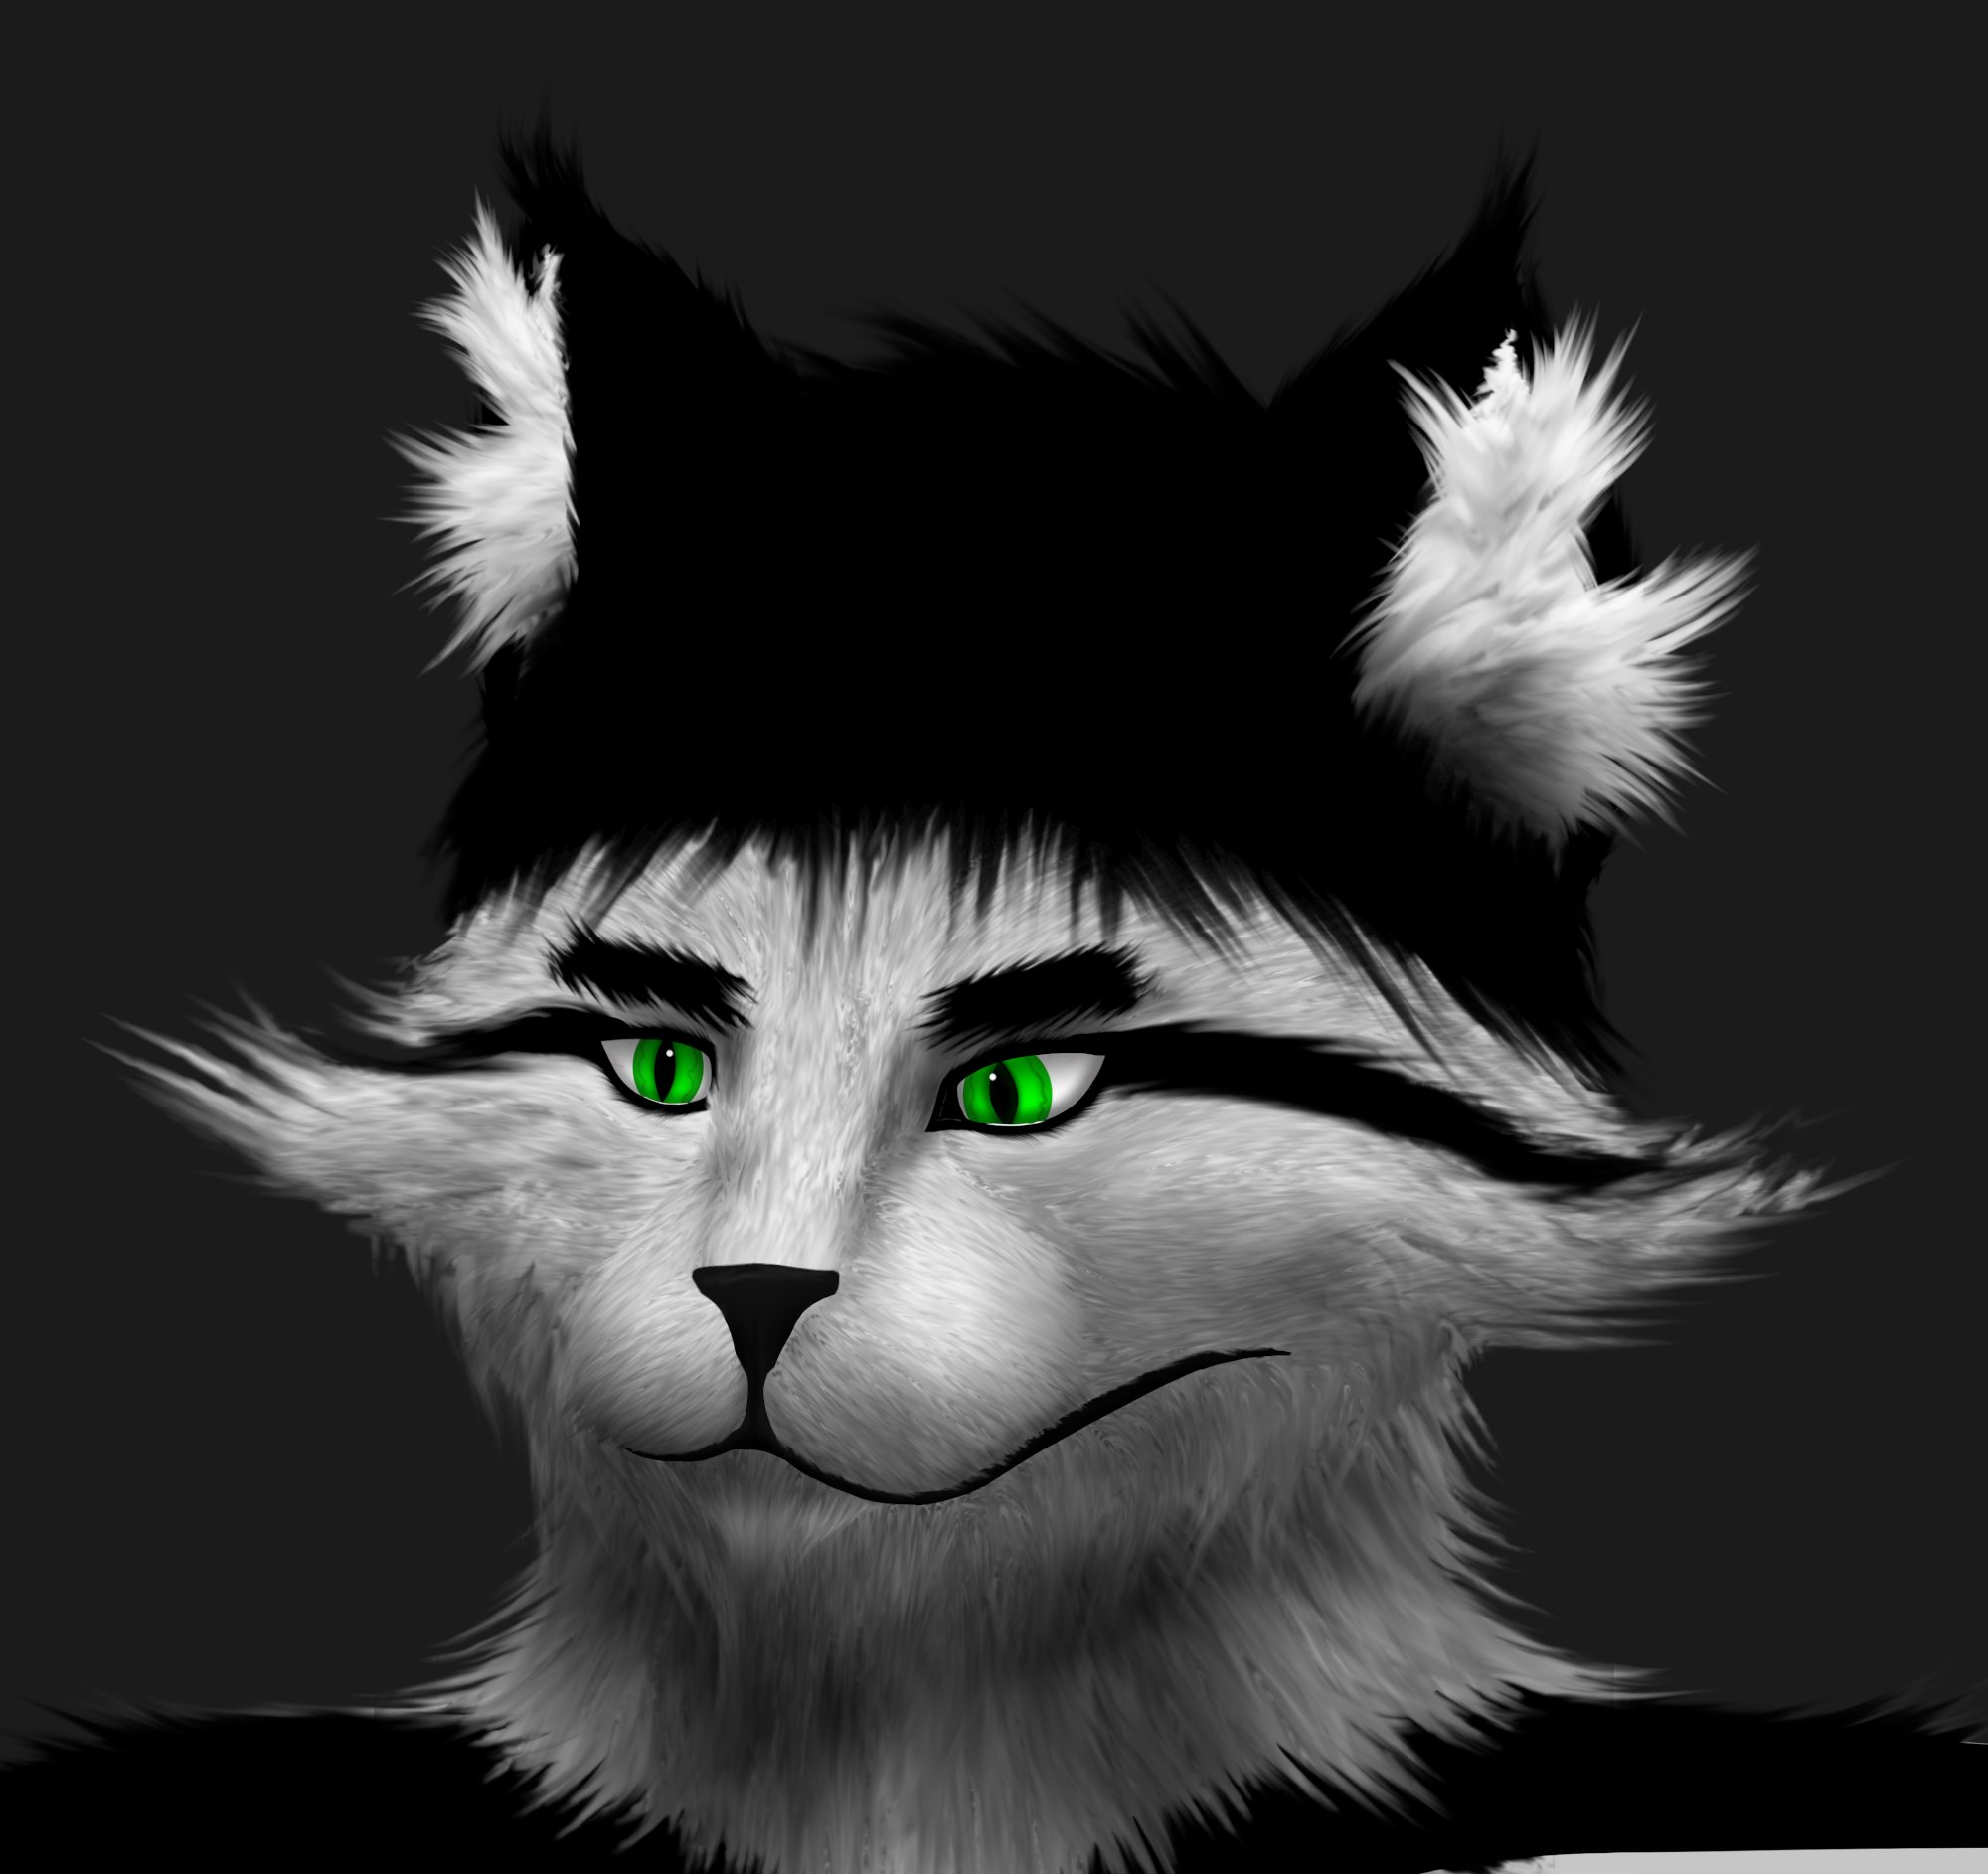
\includegraphics[width=10cm]{judastrainwreck/judastrainwreck-nohandlebars.png}
	\caption[center]{gubgau le versiio be la'oi .JUDASTRAINWRECK.\ ku poi na pixra le birka be la'oi .VUNC.}
\end{figure}
ni'o la'o gy.\ JUDASTRAINWRECK\hyp NOHANDLEBARS .gy.\ cu versiio la'oi .JUDASTRAINWRECK.\ je cu na pixra le birka be la'oi .VUNC.

\chapter{ko'a goi la'oi .THROWTHOSEPICTURESDOWNTHELANE.}
\section{le pixra}
\begin{figure}[ht]
	\centering
	\includegraphics[keepaspectratio, width=\textwidth, height=0.75\textheight]{throwthosepicturesdownthelane/throwthosepicturesdownthelane.png}
	\caption[center]{ni'o dei poi me'oi .caption.\ cu na vasru lo se xamsku}
\end{figure}
\section{le pamoi velski}
\subsection{le torveki}
ni'o la .varik.\ cu gasnu le nu fanmo le nu la .varik.\ cu zasysti le nu la .varik.\ cu terxra kei kei kei je cu gubyternoi .ui le cnino pixra

ni'o pixra le nu la'oi .VUNC.\ renro le me'oi .discus.\ poi cizra je cu xunre je cu kinli je cu te ciska le me'oi .lambda.\ poi to'alfu

ni'o la .varik.\ cu zbasu le pixra ki'u le nu la .varik.\ cu djica le nu la .varik.\ cu salci le nu la .varik.\ cu tolri'ugau le se zbasu be la .varik\ldots je cu tervenynoi la'oi .Matel.

ni'o le nu jmina lo srasu le pixra

ni'o la'o gy.\ public domain .gy.\ vasru le pixra\ldots je ro le pixra be fi la .varik.

ni'o ranji fa le nu la .varik.\ cu tervencpe lo nu nitpiki

ni'o la .varik.\ cu pilno la'oi .GIMP.\ je la'oi .OpenBSD.\ je .oiru'e .u'i le me'oi .trackpad.

\subsection{le fanmo be le nu zasysti}
ni'o la .varik.\ cu bilma je cu fliba le nu li renorere pi'e nore detri le nu la .varik.\ cu terxra kei kei ba le nu la .varik.\ cu gubyternoi le cnino pixra\sds  .i ti poi cnino pixra cu se cmene zo'oi .THROWTHOSEPICTURESDOWNTHELANE.

\subsection{le velski be le pixra}
ni'o la'oi .THROWTHOSEPICTURESDOWNTHELANE.\ pixra le nu la'oi \linebreak  % ni'o ga naja na pilno zo'oi .\linebreak.\ gi lo me'oi .\hbox.\ cu me'oi .overfull.
.VUNC.\ renro le me'oi .discus.\ poi .ue'e sinxa la'oi .Matel.\ noi samru'e je cu se zbasu la .varik.\sds  .i lo prenu poi ke'a goi ko'a zo'u cumki fa le nu la'oi .Matel.\ cinri ko'a kei ku ku goi ko'a milxe gleki le nu ko'a djuno le du'u la'oi \url{https://github.com/varikvalefor/matel} zdani pe'a le samselpla po la'oi .Matel.

\subsection{le mukti}
ni'o la .varik.\ terxra fi la'oi .THROWTHOSEPICTURESDOWNTHELANE.\ ki'u le nu la .varik.\ cu djica le nu la .varik.\ cu salci le nu la .varik.\ cu renro pe'a la'oi .Matel.\ la'o gy.\ public domain .gy.\ldots kei kei je zo'e

\subsection{le srasu}
ni'o le pixra cu pixra le srana je zo'e\sds  .i rirci fa le nu la .varik.\ cu terxra fi lo srana

ni'o la .varik.\ cu pu zu jmina le srasu le pixra

ni'o la .varik.\ cu troci le nu la .varik.\ cu jmina le srasu le pixra kei le nu la .varik.\ cu pilno le te galfi fi la .varik.\ fe le tadji be le nu la .varik.\ cu pixra loi sirsunla kei ku ku ku le nu terxra le srasu le pixra\sds  .i la .varik.\ cu na mutce le ka jinvi fi le jalge be le nu la .varik.\ cu pilno le te galfi\ldots kei kei ku'i je cu jinvi le du'u lakne fa le nu le jalge cu tcemlixau

\subsection{la'o gy.\ public domain .gy.}
ni'o la'oi .THROWTHOSEPICTURESDOWNTHELANE.\ vasru la'o gy.\ public domain .gy.\ je cu se plijaspu la'oi .Unlicense.\ noi se skicu la'o gy.\ \url{https://unlicense.org} .gy.

.i la .varik.\ cu radji'i le du'u li ni'e ni la'oi .Unlicense.\ mapti lo samru'e cu zmadu li ni'e ni la'oi .Unlicense.\ mapti lo pixra\sds  .i ku'i la .varik.\ cu pilno la'oi .Unlicense.\ ki'u le nu la .varik.\ cu nelci le nu la'oi .Unlicense.\ tordu kei je cu to'e nelci le nu la'oi .CC0.\ je zo'e cu clani

.i ji'a ro le pixra poi pu se gubyternoi la .varik.\ cu pu binxo lo se plijaspu be la'oi .Unlicense.

.i ji'a ji'a so'e lo se zbasu be la .varik.\ cu se renro pe'a fi la'o gy.\ public domain .gy.

\subsection{lo nu nitpiki}
ni'o la .varik.\ cu tervencpe lo nu nitpiki le pixra kei ku poi ke'a goi ko'a zo'u cumki fa le nu la .varik.\ cu pilno ko'a

.i si'a la .varik.\ cu na djica lo nu tcila claxu to'e nitpiki

.i lo'i mupli poi ke'a goi ko'a zo'u cumki fa le nu la .varik.\ cu pilno ko'a cu se vasru lu mi to'e nelci ti li'u noi selfilsmu lu mi to'e nelci le se pixra li'u je lu mi to'e nelci le pixra li'u

\subsection{le pilno}
ni'o .uecu'i la .varik.\ cu pilno la'oi .GIMP.\ je la'oi .OpenBSD.\ je .u'i ko'a goi le me'oi .trackpad.\ poi mutce milxe le ka mabla ku'o le nu la .varik.\ cu terxra fi la'oi .THROWTHOSEPICTURESDOWNTHELANE.\sds  .i le nu pilno ko'a le nu terxra cu fi te prali le nu lebna lo xamgu sevzi cusku noi se cinri no lo prenu

\section{le selji'i be fi ko'a}
ni'o jinvi\ldots
\begin{itemize}
	\item le du'u ko'a pixra le nu le srasu cu smimlu loi sirsunla kei kei je
	\item le du'u ko'a pixra le nu le kanla be la'oi .VUNC.\ cu claxu lo tcila kei kei je
	\item le du'u ko'a pixra le nu le birka be la'oi .VUNC.\ cu dukse le ka ce'u clani li'u kei kei kei je
	\item le du'u ko'a pixra le nu le loldi cu dukse le ka ce'u xekri kei kei kei je
	\item le du'u ko'a pixra le nu le srasu poi sarno le kacma pe'a cu dukse le ka gusni ce'u kei kei kei je
	\item le du'u ko'a pixra le nu le tuple be l'oi .VUNC.\ cu dukse le ka ce'u tordu kei kei kei je
	\item le du'u ko'a pixra le nu le dizlo zunle kinli be le nercreka pe'a po la'oi .VUNC.\ cu dukse le ka ce'u galtu kei kei kei je
	\item le du'u ko'a pixra le nu le zunle tuple be la'oi .VUNC.\ cu dukse le ka viska ce'u kei kei kei je
	\item le du'u ko'a pixra le nu le selxra xarpre cu smimlu lo sampre kei kei je
	\item le du'u ko'a pixra le nu le stedu cu dukse le ka ce'u cmalu kei kei kei je
	\item le du'u ko'a pixra le nu le xance cu dukse le ka ce'u barda kei kei kei
\end{itemize}

\subsection{le selji'i be la .varik.\ bei ko'a}
ni'o se cfifa'i la .varik.\ la'oi .THROWTHOSEPICTURESDOWNTHELANE.\ fa\ldots
\begin{itemize}
	\item le du'u la .varik.\ cu jinvi le du'u le srasu poi se pixra ko'a cu smimlu loi sirsunla kei kei je
	\item le du'u ko'a pixra le nu le kanla be la'oi .VUNC.\ cu claxu lo tcila
\end{itemize}

\subsubsection{le ka le srasu cu smimlu loi sirsunla}
ni'o la .varik.\ cu jinvi le du'u ko'a pixra le nu le srasu cu smimlu loi sirsunla kei kei je le du'u lakne le nu le ka ce'u smimlu loi sirsunla cu se rinka le nu le pu'u la .varik.\ cu terxra le srasu cu smimlu le pu'u la .varik.\ cu terxra loi sirsunla\sds  .i ku'i la .varik.\ cu cpedu lo selji'i be lo prenu poi na du la .varik.\ bei fi le srasu poi se pixra ko'a

\subsubsection{le du'u ko'a pixra le nu le kanla be la'oi .VUNC.\ cu claxu lo tcila}
ni'o ko'a vasru pare ki'o ki'o le vidnysle\footnote{.i je'au le pixra cu vasru le remu ki'o ki'o vidnysle\sds  .i ku'i vasru le toldra ki'u le nu nurbe'i}\ldots je ku'i cu claxu lo tcila be ro le kanla be la'oi .VUNC.\ ku goi ko'e\sds  .i sa'unai ko'a pixra le nu ko'e claxu lo selvi'a blutu'u je le me'oi .striation.\ pe le kalca'osrumu'a\sds  .i la .varik.\ cu jinvi le du'u dapma fi le nu ckaji le ka ce'u mo'isti

\subsection{le selji'i be lo na du be la .varik.\ be'o bei ko'a}
ni'o le su'o prenu cu cfifa'i zo'e ko'a\sds  .i la'e di'u pluka la .varik.\sds  .i le torveki be le su'o selji'i cu se mupli\ldots
\begin{itemize}
	\item lu le birka be la'oi .VUNC.\ cu dukse le ka ce'u clani li'u je
	\item lu le loldi cu dukse le ka ce'u xekri li'u je
	\item lu le srasu poi darno le kacma pe'a cu dukse le ka gusni ce'u li'u je
	\item lu le tuple be la'oi .VUNC.\ cu dukse le ka ce'u tordu li'u je
	\item lu le dizlo zunle kinli be le nercreka pe'a po la'oi .VUNC.\ cu dukse le ka ce'u galtu li'u je
	\item lu le zunle je tuple be la'oi .VUNC.\ cu dukse le ka viska ce'u li'u je
	\item lu le selxra xarpre cu smimlu lo sampre li'u je
	\item lu le stedu cu dukse le ka ce'u cmalu li'u je
	\item lu le xance cu dukse le ka ce'u barda li'u
\end{itemize}

\subsubsection{lu le birka be la'oi .VUNC.\ cu dukse le ka ce'u clani li'u}
ni'o le su'o prenu cu xusra le du'u ko'a pixra le nu le birka be le versiio be la'oi .VUNC.\ ku poi se pixra ko'a cu dukse le ka ce'u clani kei kei kei goi ko'e\sds  .i la .varik.\ cu milxe tugni fi ko'e\ldots je ku'i cu jinvi le du'u lakne fa le nu le ka le birka cu clani ku ju'anai jalge le .asna be la'oi .VUNC.\ ku poi se pixra ko'a\ldots kei kei je ku'i cu je'a radji'i le du'u cumki fa le nu le birka be la'oi .VUNC.\ cu dukse le ka ce'u clani

\subsubsection{lu le loldi cu dukse le ka ce'u xekri li'u}
ni'o le su'o prenu cu xusra ko'e goi le du'u ko'a pixra le nu le xekri je blabi poi ke'a goi ko'i zo'u ko'a pixra le nu la'oi .VUNC.\ sanli ko'i cu dukse le ka ce'u xekri\sds  .i la .varik.\ cu toltu'i fi ko'e ki'u le nu la .varik.\ se tolsnuti le nu le se sanli be la'oi .VUNC.\ cu tcetcetcexekri

\subsubsection{lu le srasu poi darno le kacma pe'a cu dukse le ka gusni ce'u li'u}
ni'o le su'o prenu cu xusra ko'e goi le du'u ko'a pixra le nu le srasu poi darno le kacma pe'a cu dukse le ka gusni ce'u kei kei kei je ko'i goi le du'u xamgu fa le nu de'i le srasu cu to'e gusybi'o\sds  .i la .varik.\ cu milxe tugni fi ko'e je ko'i

\subsubsection{lu le tuple be la'oi .VUNC.\ cu dukse le ka ce'u tordu li'u}
ni'o le su'o prenu cu xusra ko'e goi le du'u ko'a pixra le nu le tuple be la'oi .VUNC.\ be'o poi se pixra ko'a cu dukse le ka ce'u tordu\sds  .i la .varik.\ cu toltu'i fi ko'e ca le nu la .varik.\ cu ciska dei kei ki'u le nu la .varik.\ cu jinvi le du'u xamgu fa le parbi be le ni le tuple be la'oi .VUNC.\ cu clani bei le ni le torso be la'oi .VUNC.\ cu clani

\subsubsection{lu le dizlo zunle kinli be le nercreka pe'a po la'oi .VUNC.\ cu dukse le ka ce'u galtu li'u}
ni'o le su'o prenu cu xusra ko'e goi le du'u ko'a pixra le nu fo'a goi le dizlo zunle kinli be le nercreka pe'a po la'oi .VUNC.\ cu dukse le ka ce'u galtu kei kei kei je ko'i goi le du'u cadga fa le nu ciska pe'a fo'a le zunle zaglamtu'e be la'oi .VUNC.\sds  .i la .varik.\ cu tugni fi ko'e je ko'i

\subsubsection{lu le zunle tuple be la'oi .VUNC.\ cu dukse le ka viska ce'u li'u}
ni'o le su'o prenu cu xusra ko'e goi le du'u ko'a pixra le nu le zunle tuple be la'oi .VUNC.\ cu dukse le ka viska ce'u kei kei kei je ko'i goi le du'u cadga fa le nu fo'a pixra le nu le zunle tuple be la'oi .VUNC.\ cu trixe le pritu tuple be la'oi .VUNC.\sds  .i la .varik.\ cu tugni fi ko'e je ko'i

\subsubsection{lu le selxra xarpre cu smimlu lo sampre li'u}
ni'o le su'o prenu cu xusra ko'e goi le du'u ko'a pixra ko'i goi le nu la'oi .VUNC.\ se .asna fi le ka ce'u dukse bo tinsa je sampre pe'a\sds  .i la .varik.\ cu milxe tugni fi ko'e\ldots je ku'i cu xusra le du'u ko'i cu kakne le nu se xamsku je cu srana le nu lo su'o prenu cu xamsku le du'u la .varik.\ cu sampre

\subsubsection{lu le stedu cu dukse le ka ce'u cmalu li'u}
ni'o le su'o prenu cu xusra ko'e goi le du'u ko'a pixra le nu le stedu be la'oi .VUNC.\ cu dukse le ka ce'u cmalu\sds  .i la .varik.\ cu tugni fi ko'e\ldots je cu na mutce le ka ce'u tugni fi ko'e

\subsubsection{lu le xance cu dukse le ka ce'u barda li'u}
ni'o le su'o prenu cu xusra ko'e goi le du'u ko'a pixra le nu le xance be la'oi .VUNC.\ cu dukse le ka ce'u barda  .i la .varik.\ cu tugni fi ko'e ki'u le su'u ga je la .varik.\ cu te cadga fi lo nu pixra lo nu le xance be la'oi .VUNC.\ cu mleca le stedu be la'oi .VUNC.\ le ka ce'u barda gi la .varik.\ cu jinvi le du'u ko'a pixra le nu ko'a pixra le nu le xance be la'oi .VUNC.\ cu zmadu le stedu be la'oi .VUNC.\ le ka ce'u barda
\end{document}
